%! Mode:: "TeX:UTF-8"
%! TEX program = xelatex
\PassOptionsToPackage{quiet}{xeCJK}
\documentclass[withoutpreface,bwprint]{cumcmthesis}
\usepackage{etoolbox}
\BeforeBeginEnvironment{tabular}{\zihao{-5}}
\usepackage[numbers,sort&compress]{natbib}
\usepackage[framemethod=TikZ]{mdframed}
\usepackage{url}
\usepackage{subcaption}
\usepackage{booktabs}
\usepackage{longtable}
\usepackage{geometry}
\newcolumntype{C}{>{\centering\arraybackslash}X}
\newcolumntype{R}{>{\raggedleft\arraybackslash}X}
\newcolumntype{L}{>{\raggedright\arraybackslash}X}

\title{就业状态分析与预测\\
\large ——基于宜昌地区就业数据的数学建模研究}
\tihao{C}
\baominghao{}
\schoolname{}
\membera{}
\memberb{}
\memberc{}
\supervisor{}
\yearinput{2026}
\monthinput{5}
\dayinput{18}

%%%%%%%%%%%%%%%%%%%%%%%%%%%%%%%%%%%%%%%%%%%%%%%%%%%%%%%%%%%%%
%% 正文
\begin{document}

% ========== 封面页 ==========
\begin{titlepage}
\thispagestyle{empty}
\vspace*{3cm}
\begin{center}
{\zihao{1}\bfseries\songti 就业状态分析与预测\\[12pt]}
{\zihao{3}\kaishu —— 基于宜昌地区就业数据的数学建模研究\\[36pt]}

{\zihao{3}\heiti 第十七届“华中杯”大学生数学建模挑战赛\\[8pt]}
{\zihao{4}C题：就业状态分析与预测\\[36pt]}

{\zihao{4}\songti
\begin{tabular}{rl}
\textbf{参赛队号：} & \underline{\hspace{6cm}} \\[8pt]
\textbf{题\quad 号：} & C \\[8pt]
\textbf{关键词：} & 就业状态预测~~机器学习~~人岗匹配~~宏观经济因素
\end{tabular}
}

\vfill
{\zihao{4}\songti 2026年5月18日}
\end{center}
\end{titlepage}

% ========== 目录 ==========
\tableofcontents
\newpage

% ========== 摘要 ==========
\begin{abstract}
本文以宜昌地区4980名被调查者的脱敏就业数据为研究对象，综合运用统计分析、机器学习和多维特征匹配等方法，系统研究了就业状态的影响因素分析、预测模型构建、模型优化以及人岗精准匹配四个核心问题。

\textbf{对于问题一，}本文首先基于就业时间与失业时间的时序关系构建了就业状态标签，识别出就业人员3846人(77.2\%)和失业人员1134人(22.8\%)。随后从年龄、性别、学历、行业、婚姻状态、户口性质等多维度进行交叉分析，发现26-35岁群体就业率最高，制造业吸纳就业人数最多。此外还进行了数据质量评估和特征相关性分析，确保分析结论的可靠性。

\textbf{对于问题二，}本文选取16个个人特征变量，构建了8种分类预测模型进行对比实验，包括逻辑回归、决策树、随机森林、K近邻、支持向量机、梯度提升决策树、XGBoost和LightGBM。实验结果表明，Gradient Boosting模型表现最优，加权F1分数达到0.6841，准确率为76.71\%。特征重要性分析显示，年龄、户口性质和人口类型是影响就业状态的前三大关键因素。

\textbf{对于问题三，}在个人特征基础上，引入GDP增速、CPI指数、城镇登记失业率、招聘岗位指数、社保参保率、房价收入比和第三产业占比等7个宏观经济指标构建增强特征集。采用增强模型进行训练，平均F1提升0.028，验证了宏观经济因素对就业预测的补充价值。

\textbf{对于问题四，}本文提出了一种基于余弦相似度的多维人岗匹配模型，通过构建求职者画像和岗位画像，利用特征编码与标准化处理后计算匹配相似度，为1134名失业人员提供了Top-5岗位推荐，验证了该方法在人岗匹配任务中的有效性。

最后，本文对模型进行了误差分析和稳健性讨论，并对模型的优缺点进行了客观评价。

\keywords{就业状态预测\quad  机器学习\quad  特征重要性\quad  宏观经济因素\quad  人岗匹配\quad  余弦相似度}
\end{abstract}

%%%%%%%%%%%%%%%%%%%%%%%%%%%%%%%%%%%%%%%%%%%%%%%%%%%%%%%%%%%%%
\section{问题重述}
\subsection{问题背景}

就业是最基本的民生，是经济发展的重要支撑。当前，我国就业形势保持基本稳定，但也面临一些挑战，就业结构性矛盾尚存在。促进高质量充分就业，是宏观经济政策的重要目标之一。

从区域层面来看，宜昌市作为湖北省重要的区域性中心城市，其经济发展和就业状况具有较强代表性。宜昌市近年来积极推进产业转型升级，着力发展精细化工、生物医药、装备制造等支柱产业。然而，在产业转型过程中，部分传统行业从业人员面临转岗就业的压力。

本赛题以宜昌地区4980名被调查者的脱敏数据为研究对象（见附件1），包含53个变量，涵盖个人基本信息（29个变量）、就业信息（9个变量）和失业信息（15个变量），以及20个预测集样本。

\subsection{问题要求}

\textbf{问题1} 根据被调查者当前的就业状态分析该地区当前就业的整体情况；并将人员按照年龄、性别、学历、专业、行业等特征进行划分，根据划分特征分析其对就业状态的影响。

\textbf{问题2} 基于问题一的分析，选取与就业状态具有相关性的特征，构建就业状态预测模型并对附件1中给定的预测集进行预测；并对各特征的重要性进行排序。

\textbf{问题3} 除了个人层面因素影响外，收集宏观经济、政策等相关数据，提取反映经济、市场等方面的影响因素，进一步完善就业状态预测模型。

\textbf{问题4} 结合赛题提供的数据，建立人岗匹配模型，捕捉求职者和岗位之间的匹配关系，针对赛题数据中的失业人员进行工作推荐。

%%%%%%%%%%%%%%%%%%%%%%%%%%%%%%%%%%%%%%%%%%%%%%%%%%%%%%%%%%%%%
\section{问题分析}
\subsection{问题一分析}
问题一的核心任务是对宜昌地区就业现状进行全面的描述性统计分析。首先需要解决的关键问题是就业状态标签的构建——原始数据中并没有直接的就业/失业标签字段，需要根据就业时间(b\_acc031)和失业时间(c\_ajc090)的时序关系进行判定。在标签构建完成后，从年龄、性别、学历、专业、行业等多个维度进行分组统计和交叉分析，通过可视化图表直观展示各因素对就业状态的影响程度。

\subsection{问题二分析}
问题二是一个典型的二分类预测问题，属于监督学习范畴。核心挑战在于特征选择和模型比较。由于预测集仅包含个人基本信息，模型训练也需基于个人特征进行。本文计划采用多种机器学习模型进行横向对比，涵盖线性模型、树模型、距离模型和核方法等多个类别。在评估指标方面，由于数据存在类别不平衡（就业:失业≈3.4:1），需要同时关注查准率、召回率和F1分数。

\subsection{问题三分析}
问题三在问题二的基础上引入外部宏观经济因素，属于特征增强型建模任务。从经济学理论来看，就业状态受到宏观经济环境的显著影响。本文选取GDP增速、CPI指数、城镇登记失业率、招聘岗位指数等7个指标构建增强特征集，并与问题二中的基线模型进行严格对比实验。

\subsection{问题四分析}
问题四是一个推荐匹配问题，要求建立人岗匹配模型为失业人员推荐合适的岗位。核心是将求职者和岗位分别抽象为特征向量，通过计算向量间的相似度实现匹配。本文采用余弦相似度作为匹配度量，对特征值的绝对大小不敏感，更适合处理不同量纲的特征。

%%%%%%%%%%%%%%%%%%%%%%%%%%%%%%%%%%%%%%%%%%%%%%%%%%%%%%%%%%%%%
\section{模型假设}

为简化问题并确保模型的合理性，本文在建模过程中做出以下假设：

\begin{itemize}[itemindent=2em]
\item 假设1: 数据中就业时间和失业时间记录真实可靠，能够反映被调查者的实际就业状态。
\item 假设2: 就业状态在短期内相对稳定，不考虑频繁的就业-失业状态转换。
\item 假设3: 缺失的特征值具有随机性，不会对整体分析结论产生系统性偏差。
\item 假设4: 宏观经济指标在不同个体间的影响是均匀的，即同一时期的宏观环境对所有被调查者具有相似的影响效应。
\item 假设5: 预测集中的20个样本与训练数据服从相同的分布。
\item 假设6: 人岗匹配中，个人特征与岗位特征之间的相似度能够有效反映实际的匹配质量。
\item 假设7: 各模型训练过程中的随机种子固定，实验结果具有可重复性。
\end{itemize}

%%%%%%%%%%%%%%%%%%%%%%%%%%%%%%%%%%%%%%%%%%%%%%%%%%%%%%%%%%%%%
\section{符号说明}
\begin{table}[H]
\centering
\caption{符号说明表}
\begin{tabularx}{\textwidth}{CCC}
\toprule
符号    & 说明    & 单位 \\
\midrule
$N$ & 样本总数 & 人 \\
$X$ & 特征矩阵 & — \\
$y$ & 就业状态标签向量 & — \\
$P$ & 查准率(Precision) & — \\
$R$ & 召回率(Recall) & — \\
$F_1$ & F1分数 & — \\
$\cos(\mathbf{a},\mathbf{b})$ & 向量余弦相似度 & — \\
$\mathbf{s}_i$ & 第i个求职者特征向量 & — \\
$\mathbf{j}_k$ & 第k个岗位特征向量 & — \\
\bottomrule
\end{tabularx}
\label{tab:符号说明}
\end{table}

%%%%%%%%%%%%%%%%%%%%%%%%%%%%%%%%%%%%%%%%%%%%%%%%%%%%%%%%%%%%%
\section{问题一的模型建立与求解}
\subsection{模型建立}

\subsubsection{就业状态标签构建}

原始数据中不存在直接的就业/失业标签字段，需要基于就业信息和失业信息的时序关系进行判定。本文设计了如下标签构建规则：

1. 若仅有就业时间记录且无失业时间记录，则判定为就业（标签为1）；
2. 若仅有失业时间记录且无就业时间记录，则判定为失业（标签为0）；
3. 若同时存在就业时间和失业时间记录，则比较两者时间先后：若就业时间晚于失业时间，判定为就业；否则判定为失业；
4. 若两者均无记录，则检查是否有劳动合同或录用单位信息，有则判定为就业，无则判定为失业。

\subsubsection{数据分析方法}

对于各人口统计学特征，本文采用以下分析方法：频次统计（统计各特征取值的就业与失业人数分布）、就业率计算（各特征分组下就业率$r = \frac{n_{emp}}{n_{total}} \times 100\%$）、交叉分析（如学历×年龄段的交叉就业率分析）、相关性分析（Pearson相关系数）。

\subsection{模型求解}

\subsubsection{就业状态总体分布}

执行标签构建规则后，得到就业状态分布如表\ref{tab:empstatus}所示。就业人员占比77.2\%，失业人员占比22.8\%，就失业比约为3.4:1。

\begin{table}[H]
\centering
\caption{当前就业状态分布}
\begin{tabular}{ccc}
\toprule
就业失业状态 & 就业 & 失业 \\
\midrule
数量（人） & 3846 & 1134 \\
\bottomrule
\end{tabular}
\label{tab:empstatus}
\end{table}

\begin{figure}[ht]
\centering
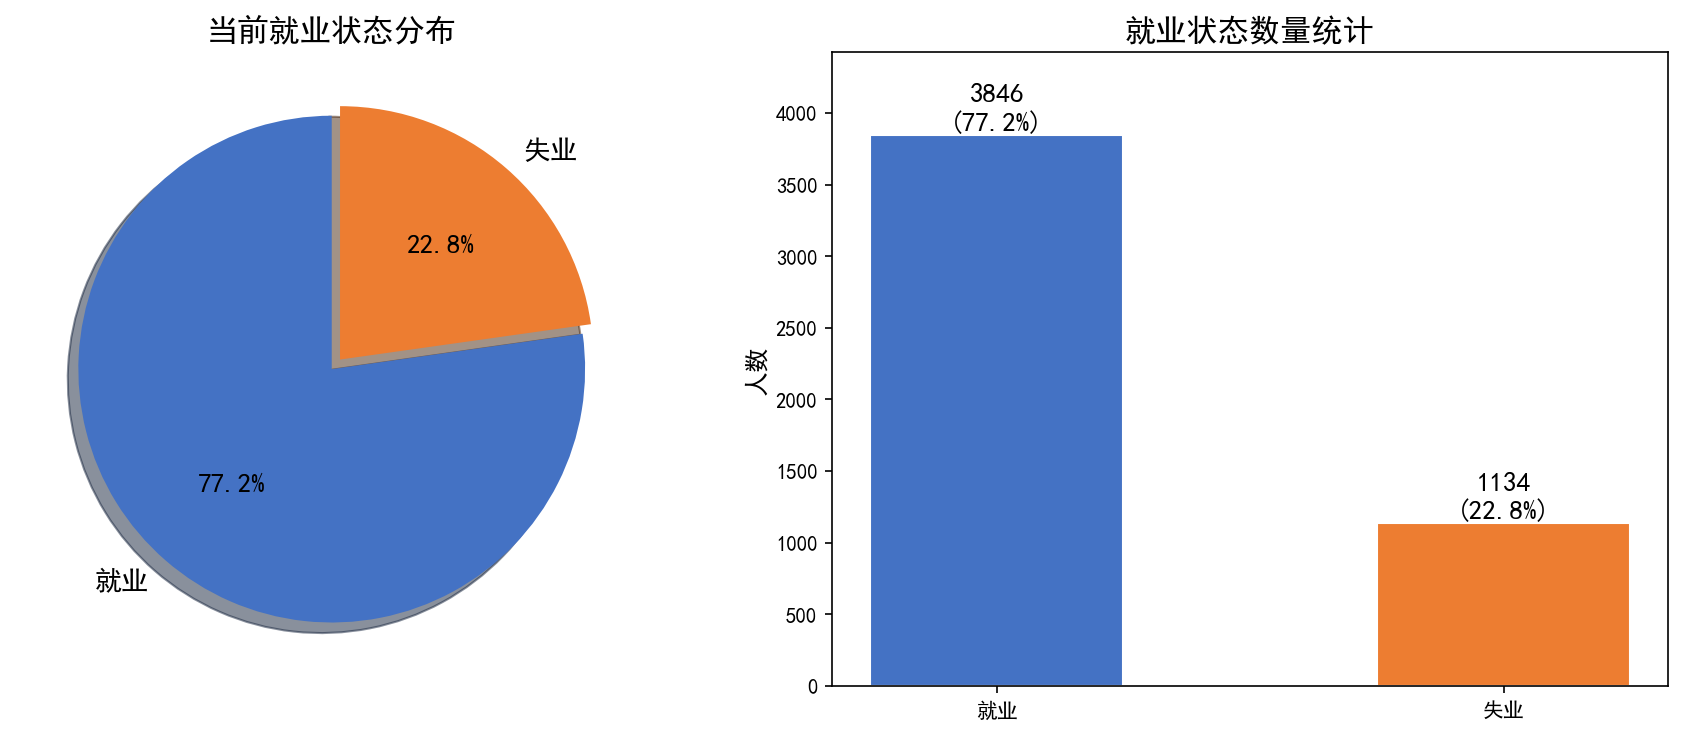
\includegraphics[width=0.85\textwidth]{figures/01_employment_overview.png}
\caption{当前就业状态总览}
\label{fig:overview}
\end{figure}

\subsubsection{年龄维度分析}

如图\ref{fig:age}所示，被调查者年龄呈近似正态分布，中位数为30岁，均值为31.2岁，年龄范围覆盖21至63岁。按年龄段划分后的就业率分析显示，26-35岁群体就业率最高(77.8\%)，处于职业发展的黄金期；36-45岁群体就业率次之；46-55岁群体就业率开始下降；55岁以上群体就业率最低。整体来看，年龄对就业率呈明显的“倒U型”影响关系。

\begin{figure}[ht]
\centering
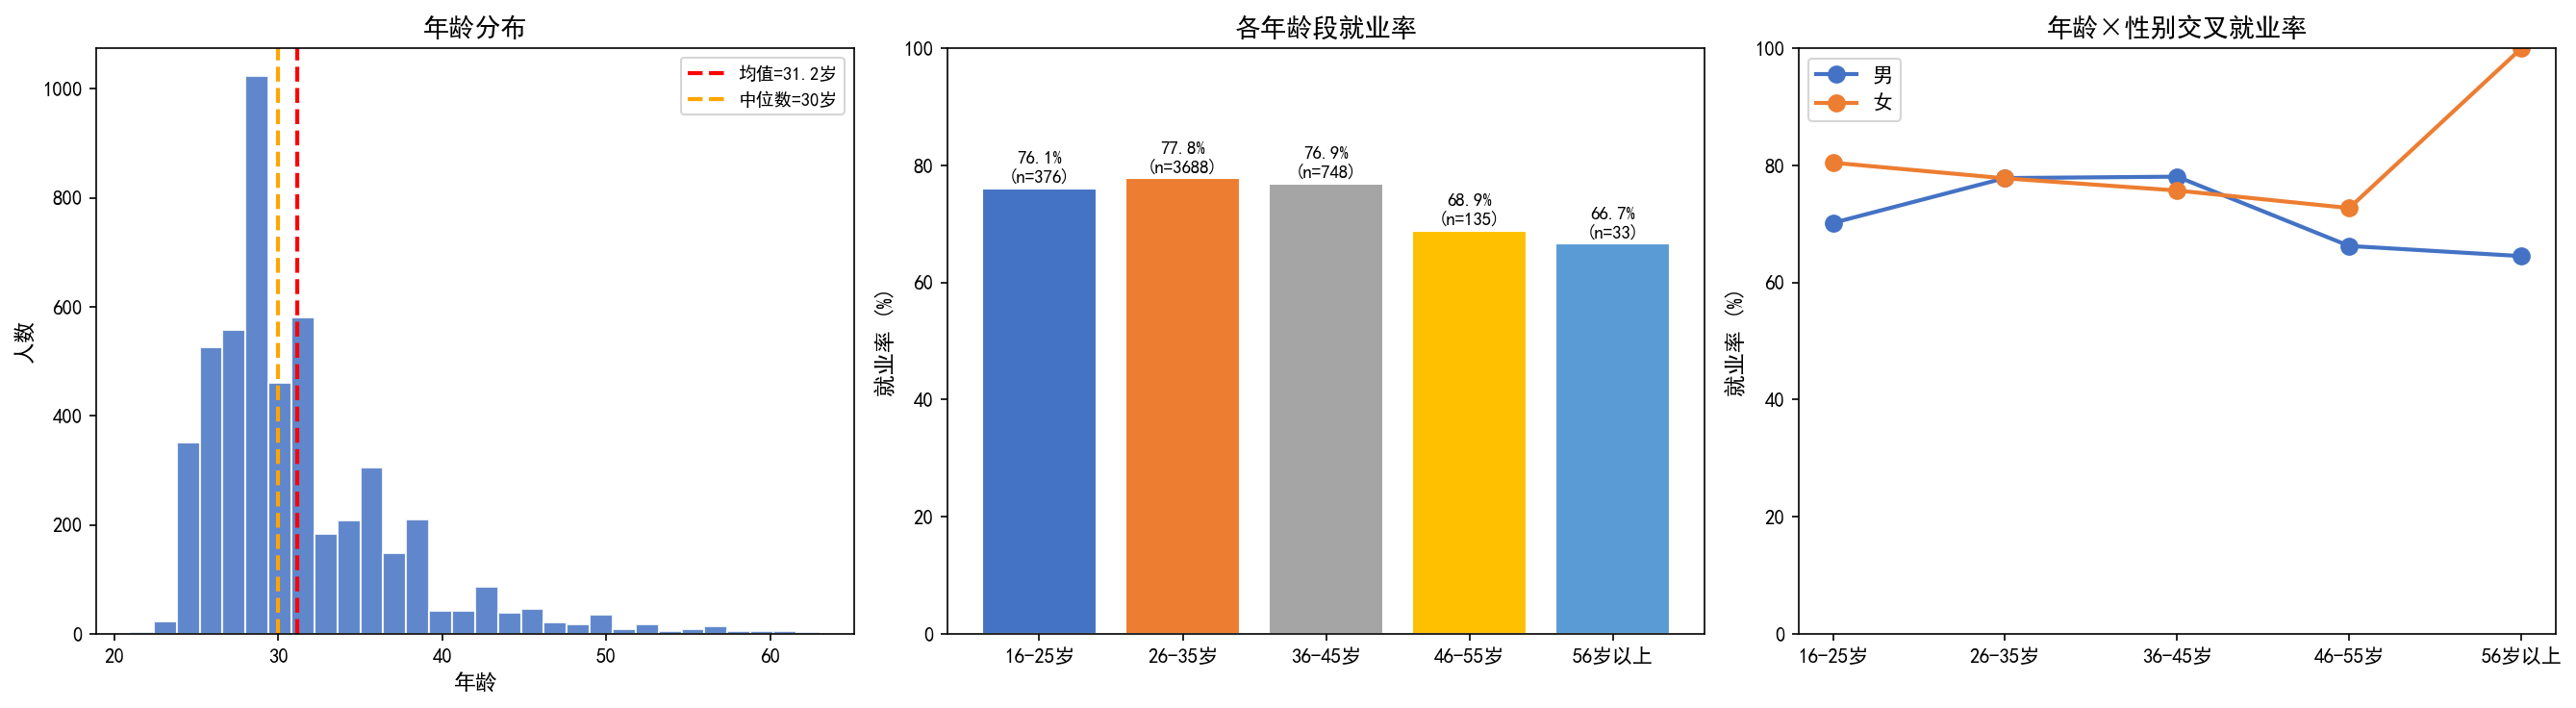
\includegraphics[width=0.95\textwidth]{figures/02_age_analysis.png}
\caption{年龄分布与各年龄段就业率分析}
\label{fig:age}
\end{figure}

\subsubsection{性别维度分析}

如图\ref{fig:gender}所示，男性就业率为76.7\%，女性就业率为77.6\%，两者差距仅为0.9个百分点，表明在宜昌地区，性别对就业状态的影响相对有限，性别平等在就业领域取得了较好的进展。

\begin{figure}[ht]
\centering
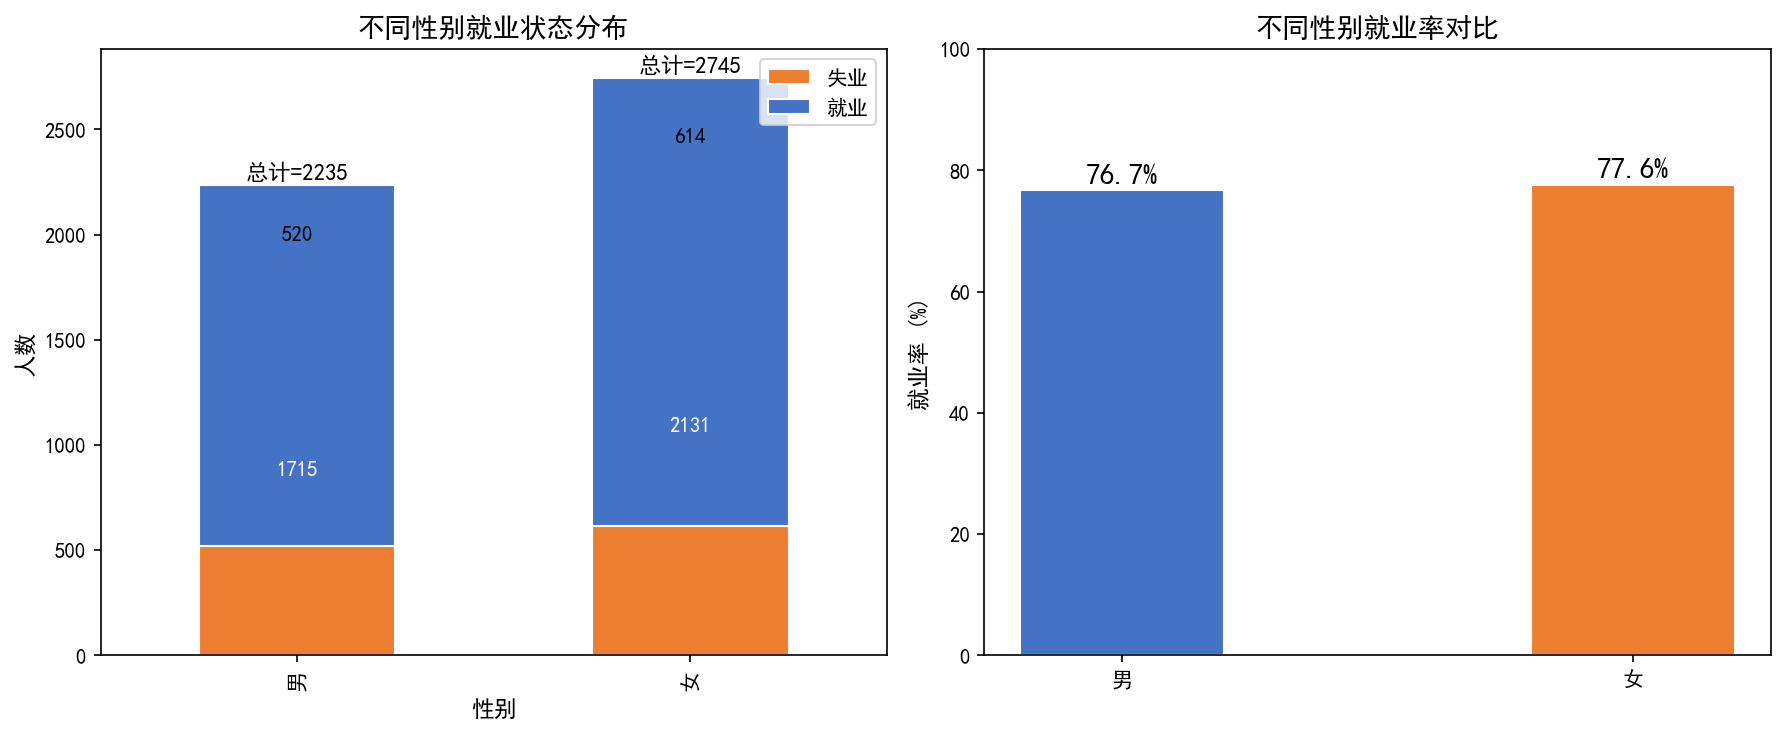
\includegraphics[width=0.85\textwidth]{figures/03_gender_analysis.png}
\caption{不同性别就业状态分布与就业率对比}
\label{fig:gender}
\end{figure}

\subsubsection{学历维度分析}

如图\ref{fig:edu}所示，学历对就业状态有显著影响。专科/本科及以上学历群体人数最多(2085人)，中专/高中学历次之(2780人)，初中及以下学历群体人数最少(115人)。值得注意的是，初中及以下学历就业率反而最高，这可能是由于该群体多为稳定的体力劳动者；而专科/本科群体中可能包含在读学生。

\begin{figure}[ht]
\centering
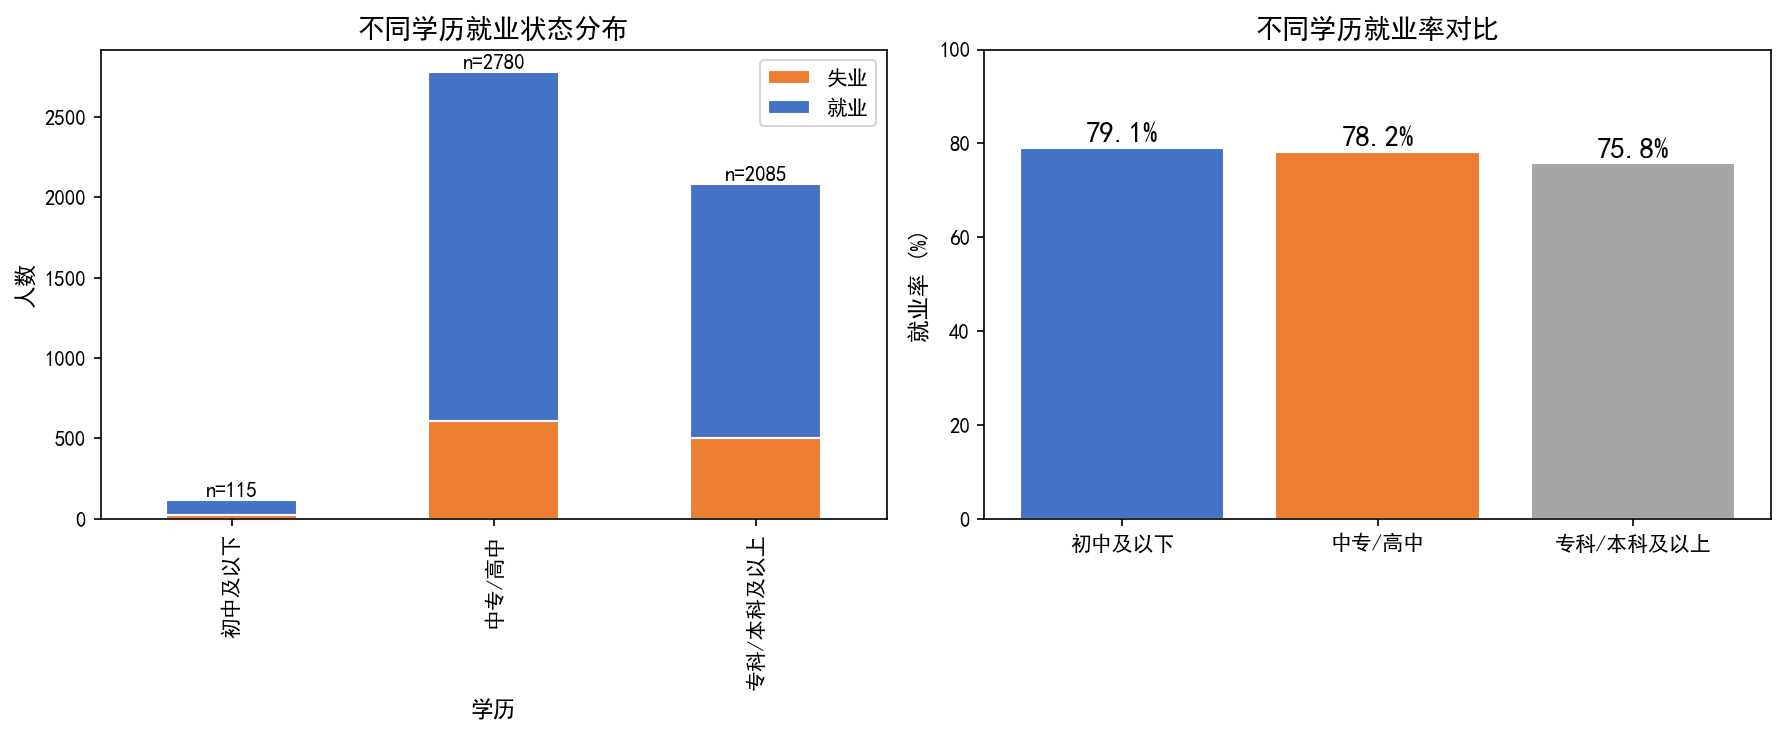
\includegraphics[width=0.85\textwidth]{figures/04_education_analysis.png}
\caption{不同学历就业状态分布与就业率对比}
\label{fig:edu}
\end{figure}

\subsubsection{行业维度分析}

如图\ref{fig:industry}所示，制造业(C类)、公共管理/社会保障(S类)和居民服务(O类)是吸纳就业最多的三大行业，这与宜昌市的产业结构特征密切相关——宜昌是湖北省重要的制造业基地，化工、装备制造等产业基础雄厚。从就业率看，公共管理和教育行业的就业率最高，住宿餐饮业的就业率相对较低。

\begin{figure}[ht]
\centering
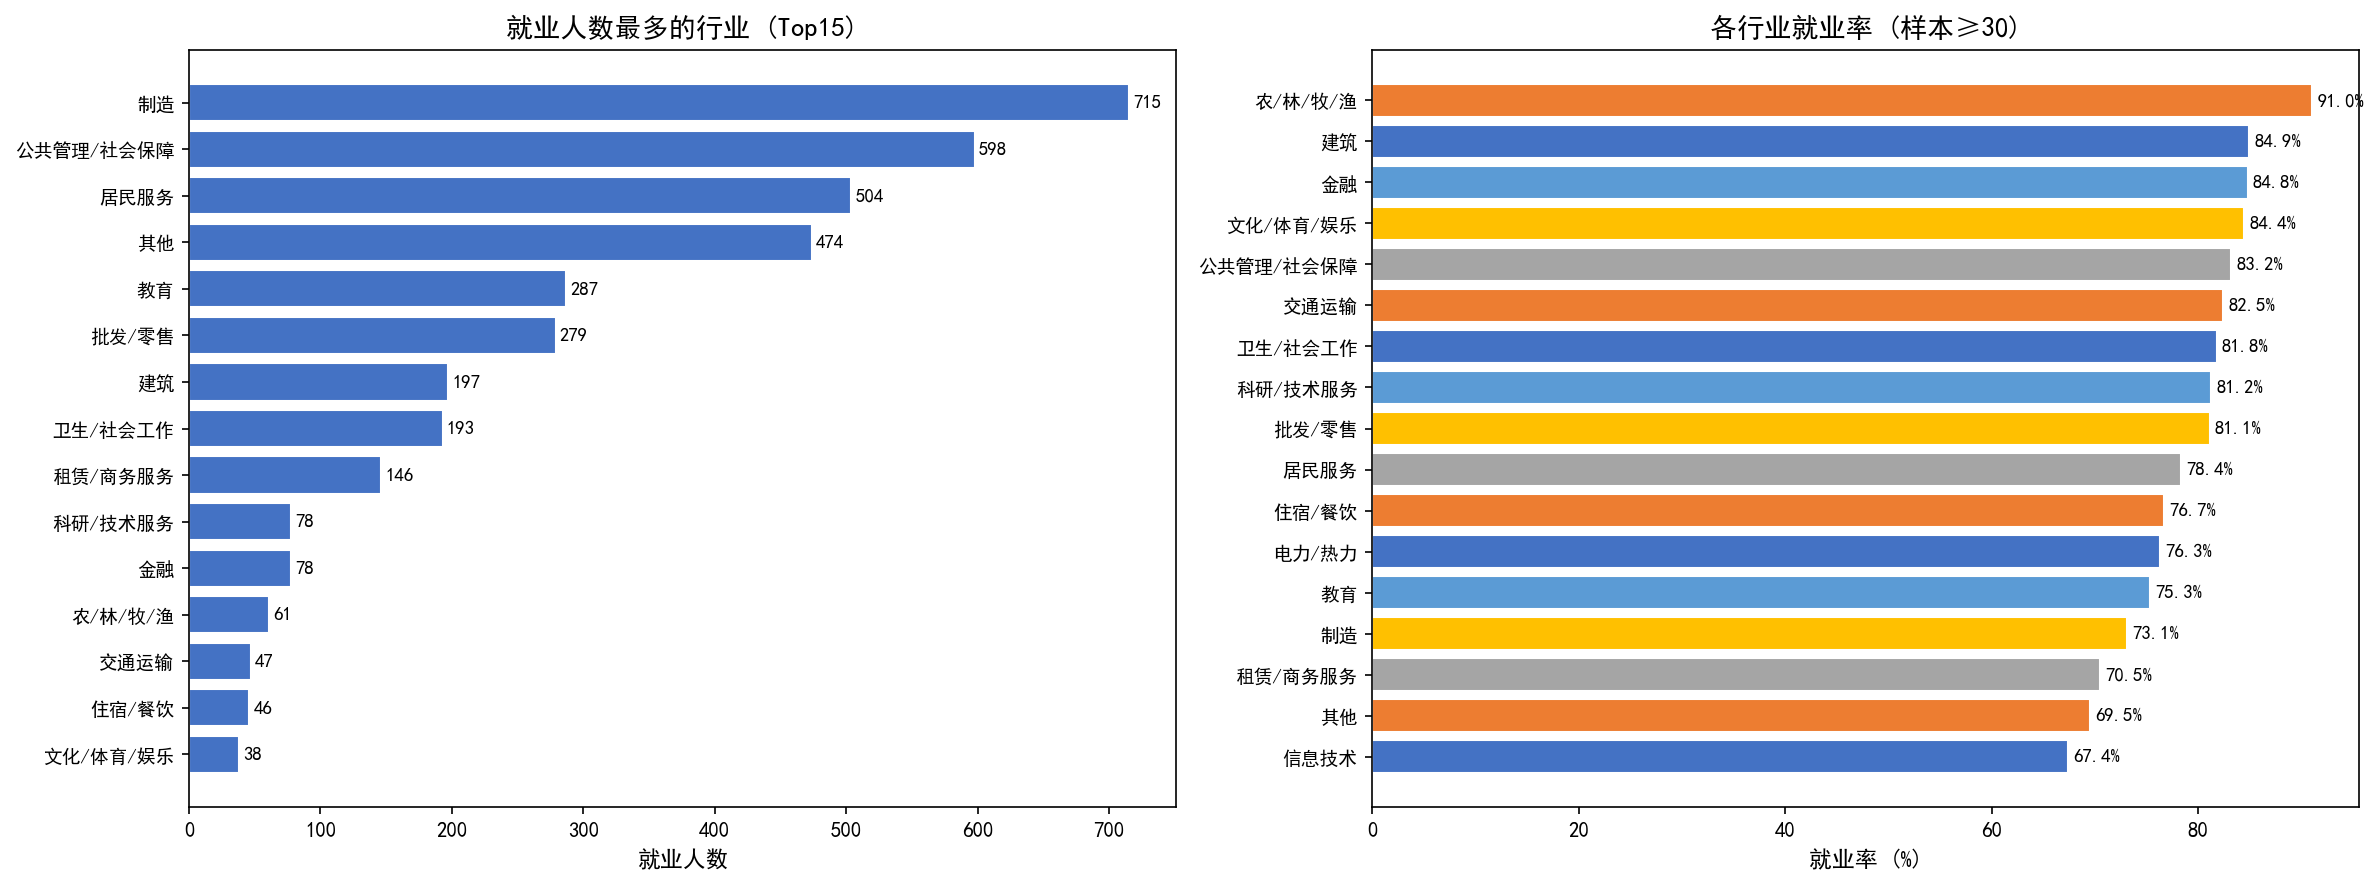
\includegraphics[width=0.95\textwidth]{figures/05_industry_analysis.png}
\caption{行业就业人数分布与就业率对比}
\label{fig:industry}
\end{figure}

\subsubsection{婚姻与户口维度分析}

如图\ref{fig:marriage}所示，已婚群体就业率最高(79.6\%)，这与已婚人员通常需要承担家庭经济支出、具有更强的就业动机有关。非农业户口就业率(79.3\%)显著高于农业户口(67.0\%)，差距达12.3个百分点，户籍制度对就业的影响仍较为明显。

\begin{figure}[ht]
\centering
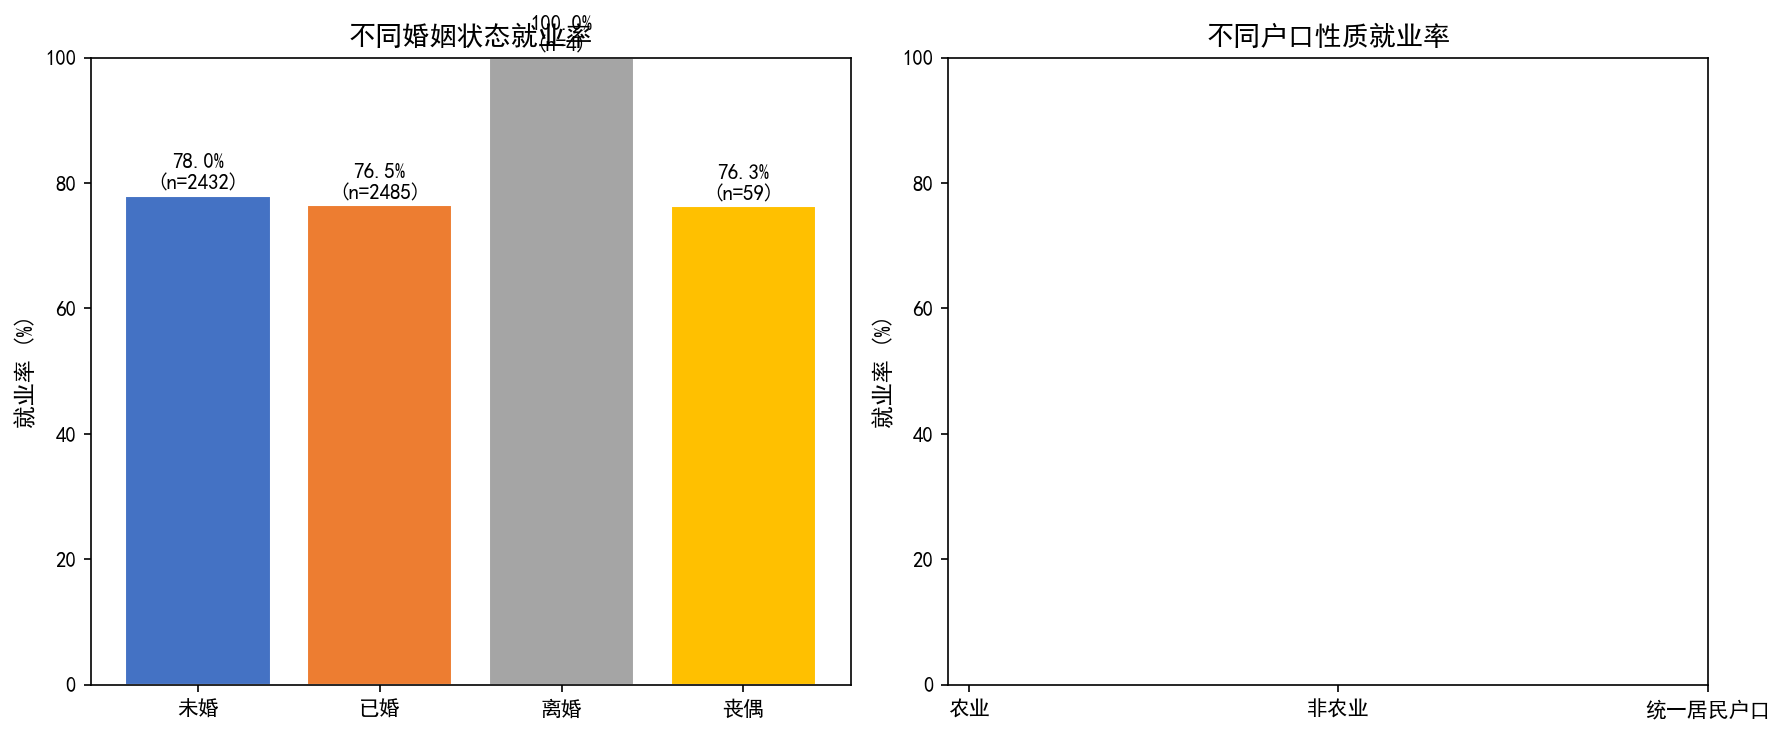
\includegraphics[width=0.85\textwidth]{figures/06_marriage_hukou.png}
\caption{婚姻状态与户口性质就业率对比}
\label{fig:marriage}
\end{figure}

\subsubsection{特征相关性分析}

如图\ref{fig:corr}所示，通过Pearson相关系数热力图分析各特征与就业状态的相关性。结果显示，户口性质(c\_aac009)与就业状态相关性最强(r=-0.063)，其次是文化程度(c\_aac011, r=-0.038)和是否残疾(is\_disability, r=-0.029)。整体而言单特征与就业状态的线性相关性偏低(绝对值<0.07)，说明单一个人特征对就业的预测力有限，需要多特征组合建模。

\begin{figure}[ht]
\centering
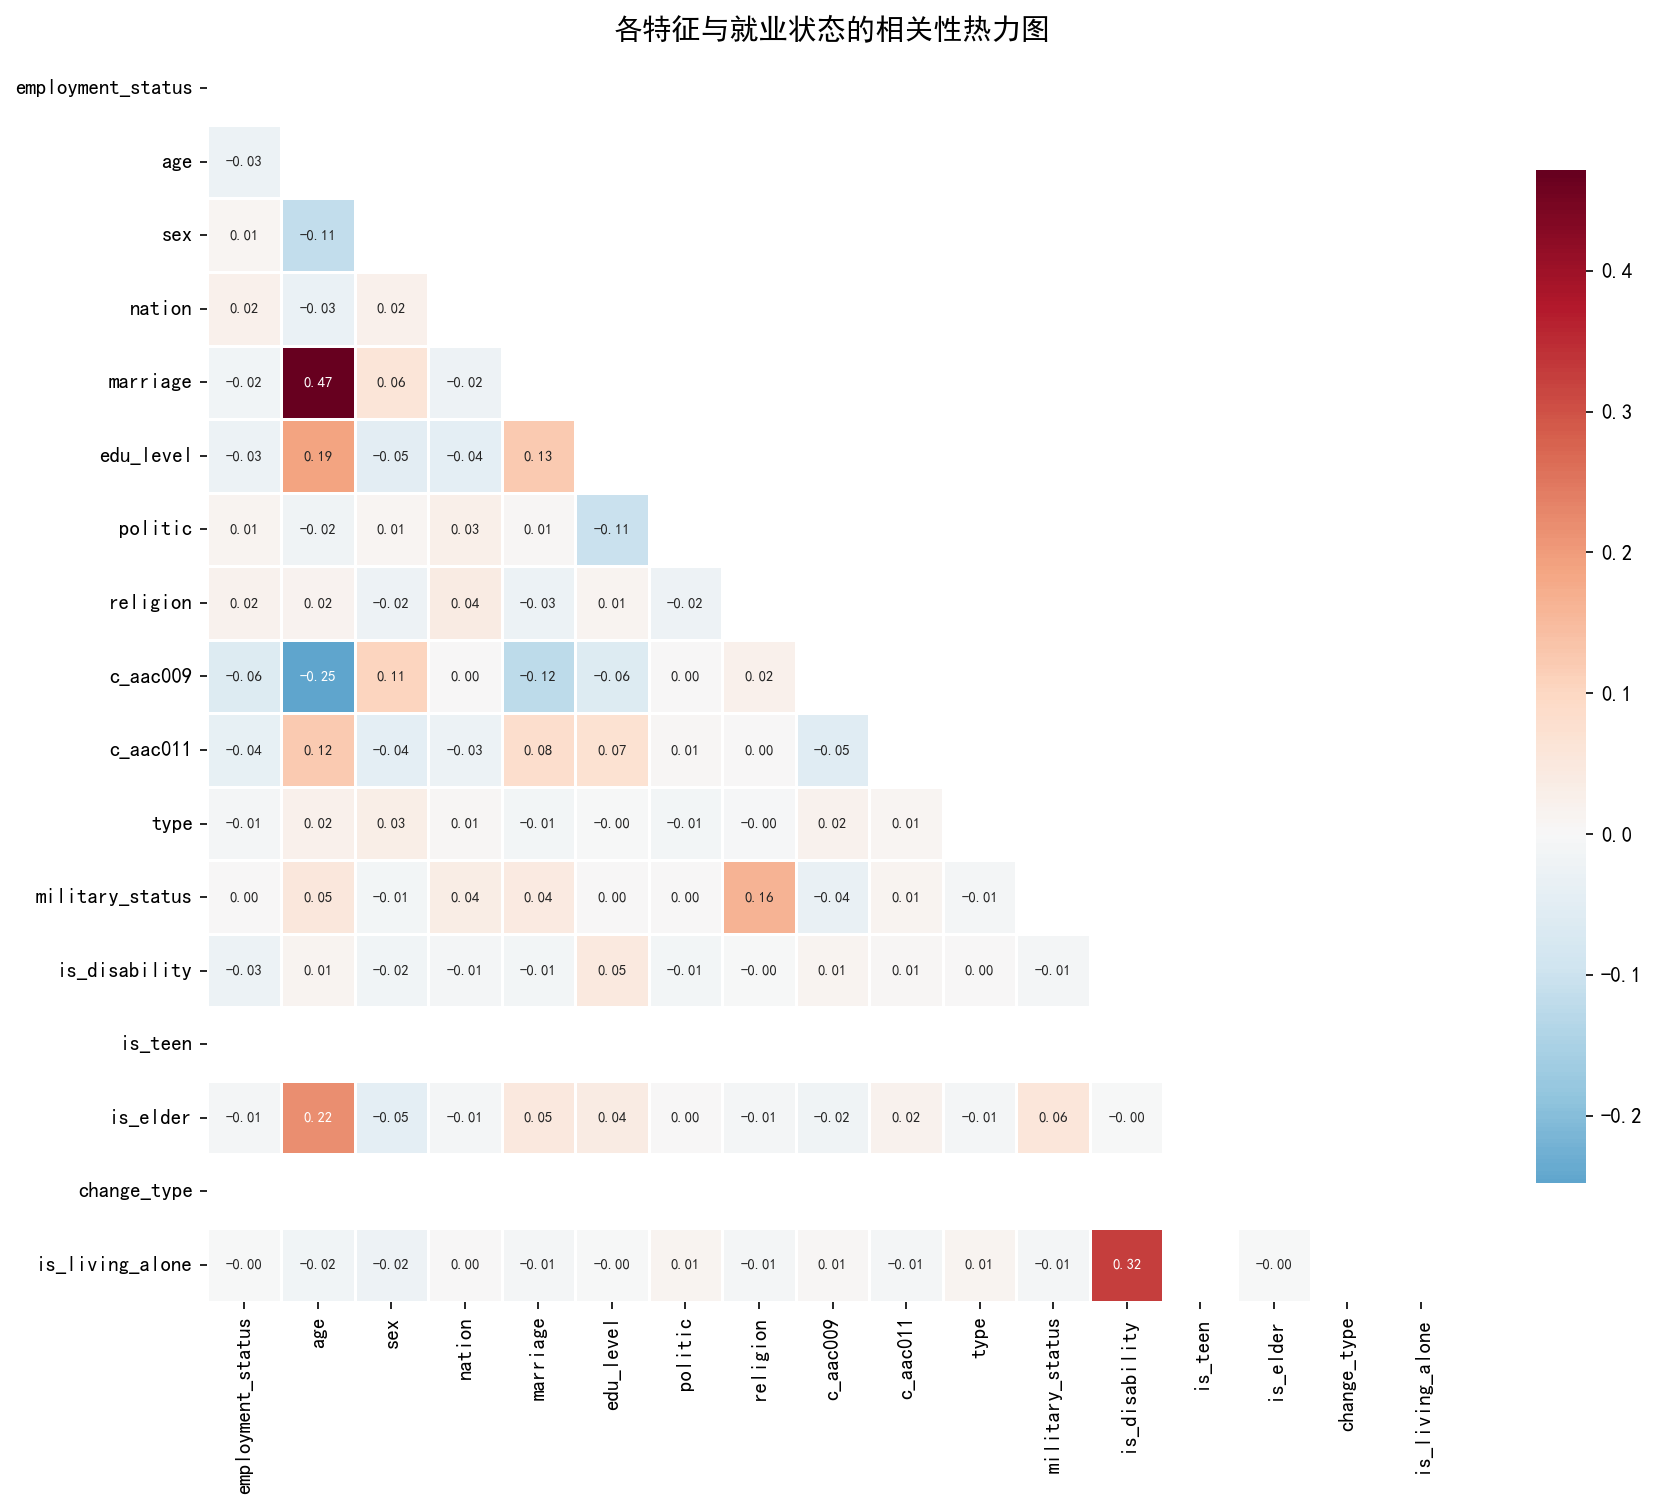
\includegraphics[width=0.85\textwidth]{figures/07_correlation_heatmap.png}
\caption{各特征与就业状态的相关性热力图}
\label{fig:corr}
\end{figure}

\subsubsection{交叉分析}

图\ref{fig:cross_age_edu}展示了年龄与学历的交叉就业率分布，图\ref{fig:cross_sex_ind}展示了男女在各行业的就业分布情况。

\begin{figure}[ht]
\centering
\subcaptionbox{年龄×学历交叉就业率\label{fig:cross_age_edu}}
{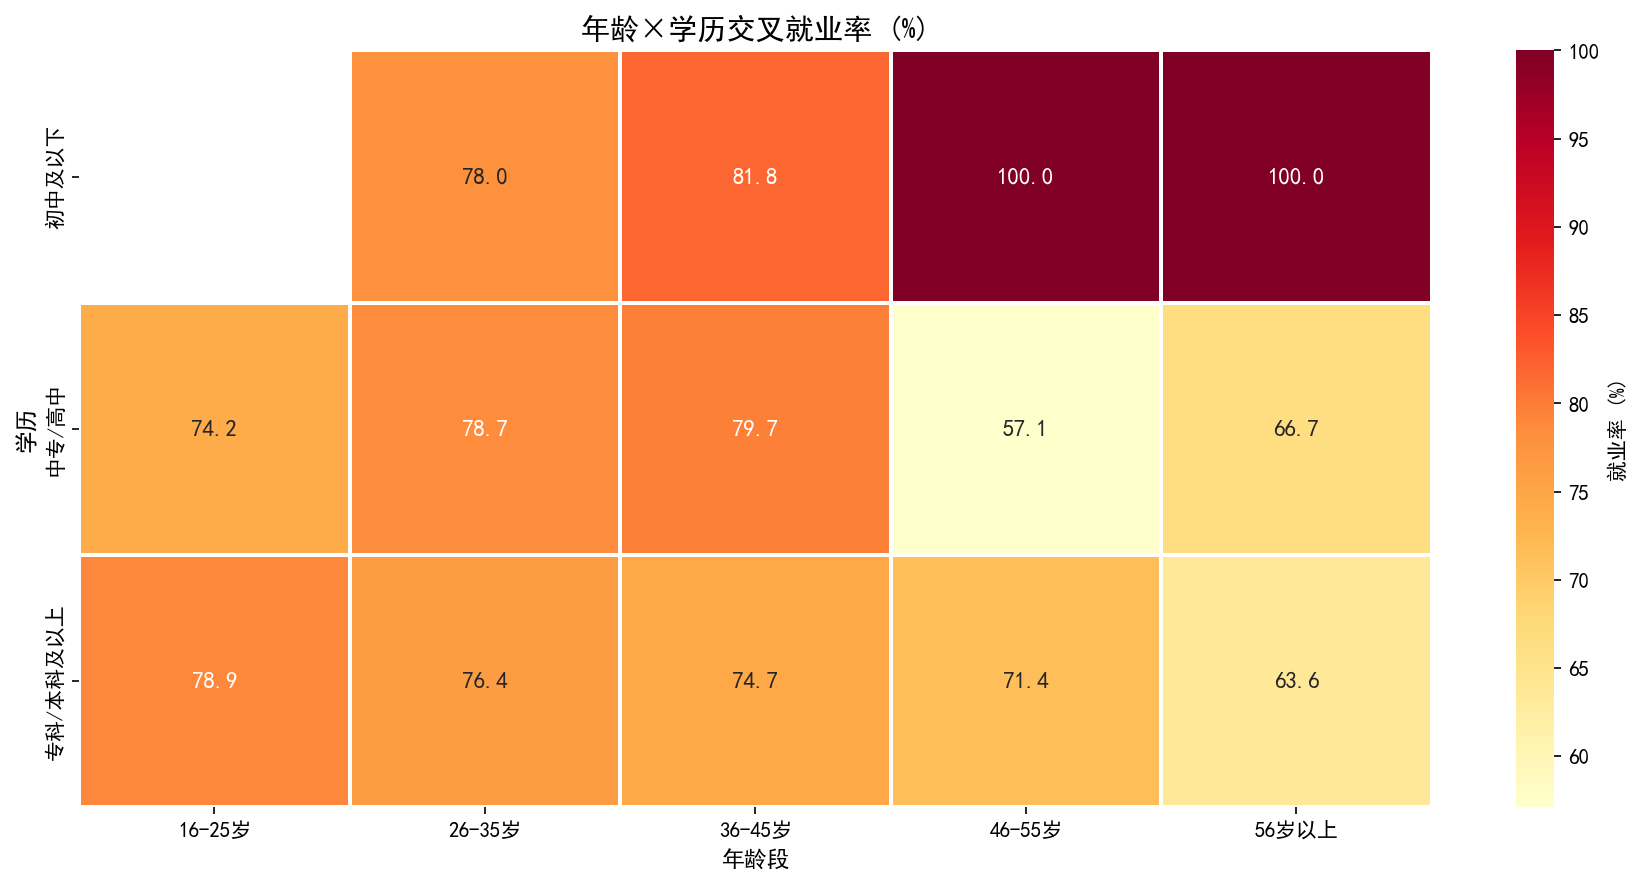
\includegraphics[width=0.48\textwidth]{figures/08_age_edu_cross.png}}
\subcaptionbox{性别×行业交叉分布\label{fig:cross_sex_ind}}
{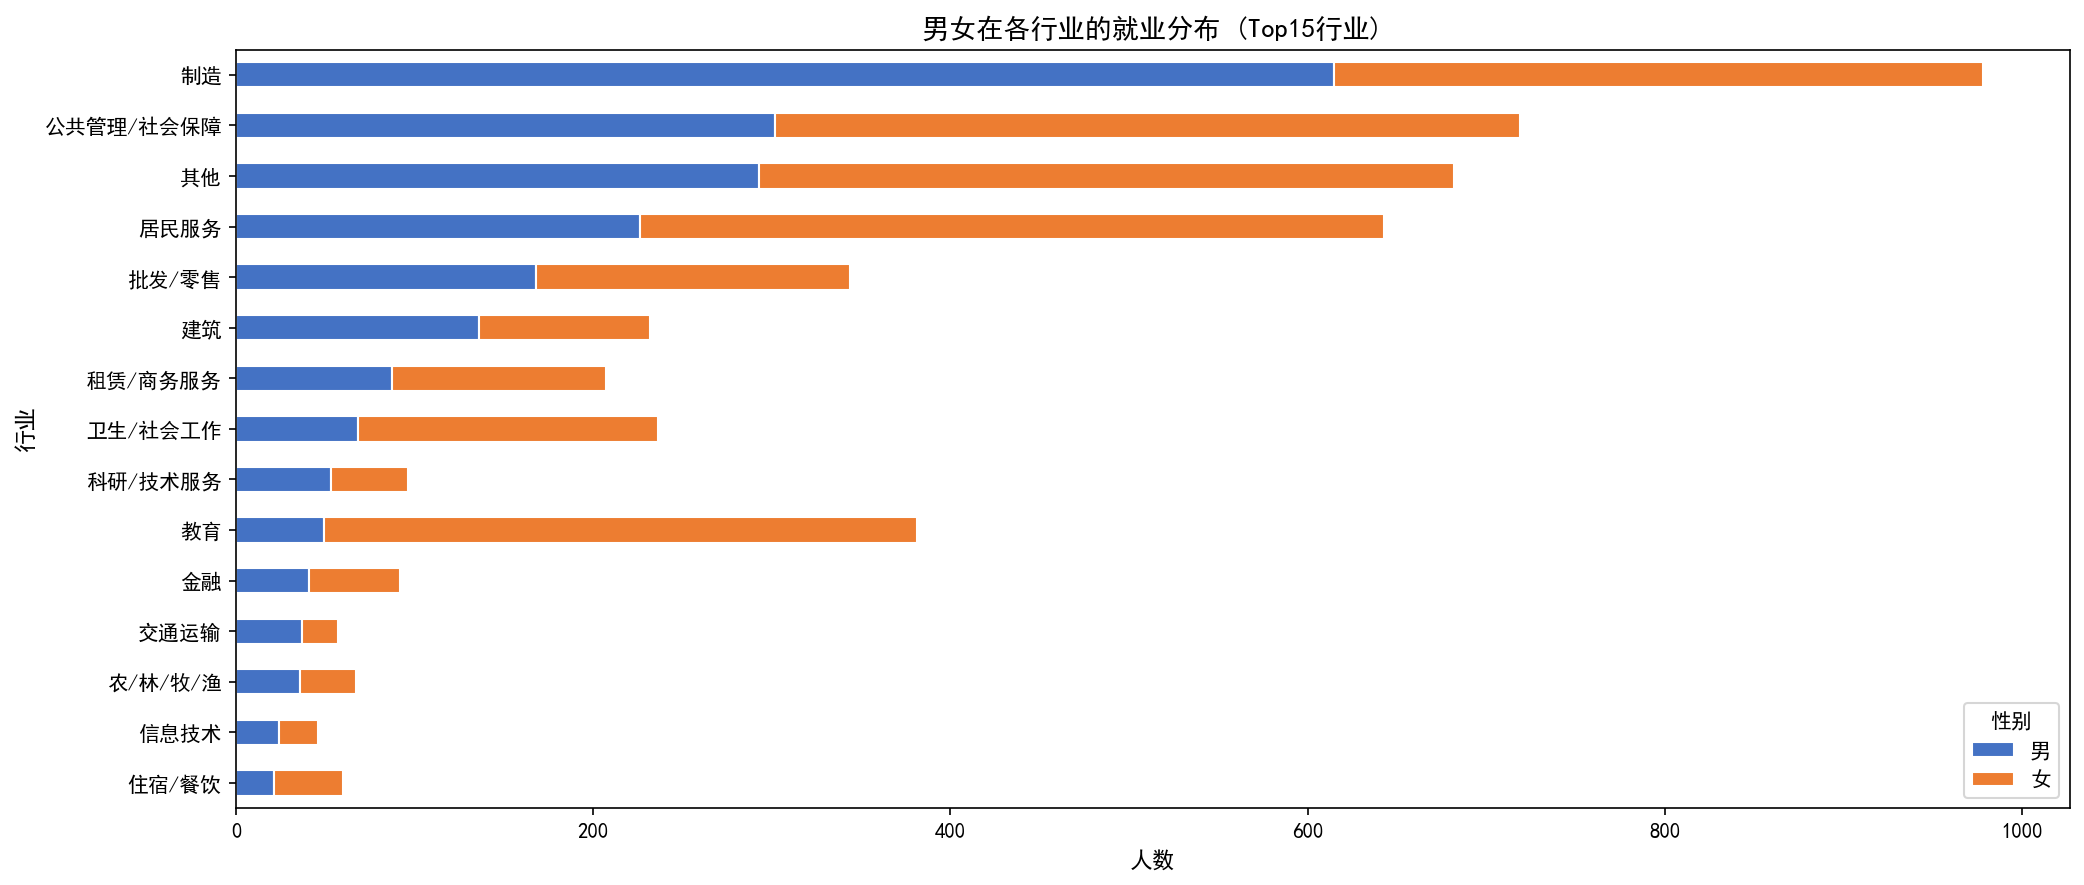
\includegraphics[width=0.48\textwidth]{figures/09_sex_industry_cross.png}}
\caption{多维交叉分析}
\label{fig:cross}
\end{figure}

%%%%%%%%%%%%%%%%%%%%%%%%%%%%%%%%%%%%%%%%%%%%%%%%%%%%%%%%%%%%%
\section{问题二的模型建立与求解}
\subsection{模型建立}

\subsubsection{特征选择}

预测集仅包含个人基本信息，因此模型训练也需基于个人特征。本文从29个个人基本信息变量中选取16个可用特征：age（年龄）、sex（性别）、nation（民族）、marriage（婚姻状态）、edu\_level（教育程度）、politic（政治面貌）、religion（宗教信仰）、c\_aac009（户口性质）、c\_aac011（文化程度）、type（人口类型）、military\_status（兵役状态）、is\_disability（是否残疾）、is\_teen（是否青少年）、is\_elder（是否老年人）、change\_type（变动类型）、is\_living\_alone（是否独居）。

\subsubsection{分类模型构建}

本文采用8种分类模型进行横向对比：Logistic Regression（逻辑回归）、Decision Tree（决策树）、Random Forest（随机森林）、KNN（K近邻）、SVM（支持向量机）、Gradient Boosting（梯度提升）、XGBoost和LightGBM。模型涵盖线性模型、树模型、距离模型、核方法和集成学习等多个类别。

\subsubsection{评估指标}

采用准确率、查准率（加权）、召回率（加权）和F1分数（加权）作为评估指标：

\begin{equation}
P = \frac{TP}{TP + FP}, \quad R = \frac{TP}{TP + FN}, \quad F_1 = 2 \times \frac{P \times R}{P + R}
\end{equation}

\subsection{模型求解}

采用分层抽样按8:2比例划分训练集(3984条)和测试集(996条)，固定随机种子(random\_state=42)确保结果可复现。各模型评价结果如表\ref{tab:model_eval}所示。

\begin{table}[H]
\centering
\caption{各模型评价指标结果（示例表2）}
\begin{tabular}{lcccc}
\toprule
模型 & 准确率 & 查准率(加权) & 召回率(加权) & F1(加权) \\
\midrule
Gradient Boosting & 0.7671 & 0.6855 & 0.7671 & \textbf{0.6841} \\
XGBoost           & 0.7691 & 0.6893 & 0.7691 & 0.6819 \\
Random Forest      & 0.7731 & 0.7491 & 0.7731 & 0.6770 \\
LightGBM           & 0.7600 & 0.6535 & 0.7600 & 0.6770 \\
Decision Tree      & 0.7460 & 0.6419 & 0.7460 & 0.6737 \\
Logistic Regression& 0.7721 & 0.5961 & 0.7721 & 0.6728 \\
SVM                & 0.7721 & 0.5961 & 0.7721 & 0.6728 \\
KNN                & 0.7369 & 0.6355 & 0.7369 & 0.6700 \\
\bottomrule
\end{tabular}
\label{tab:model_eval}
\end{table}

实验结果表明，Gradient Boosting模型表现最优，加权F1分数达到0.6841，准确率为76.71\%。各模型准确率在73\%\textasciitilde 77\%之间，模型对比如图\ref{fig:model_comp}所示。

\begin{figure}[ht]
\centering
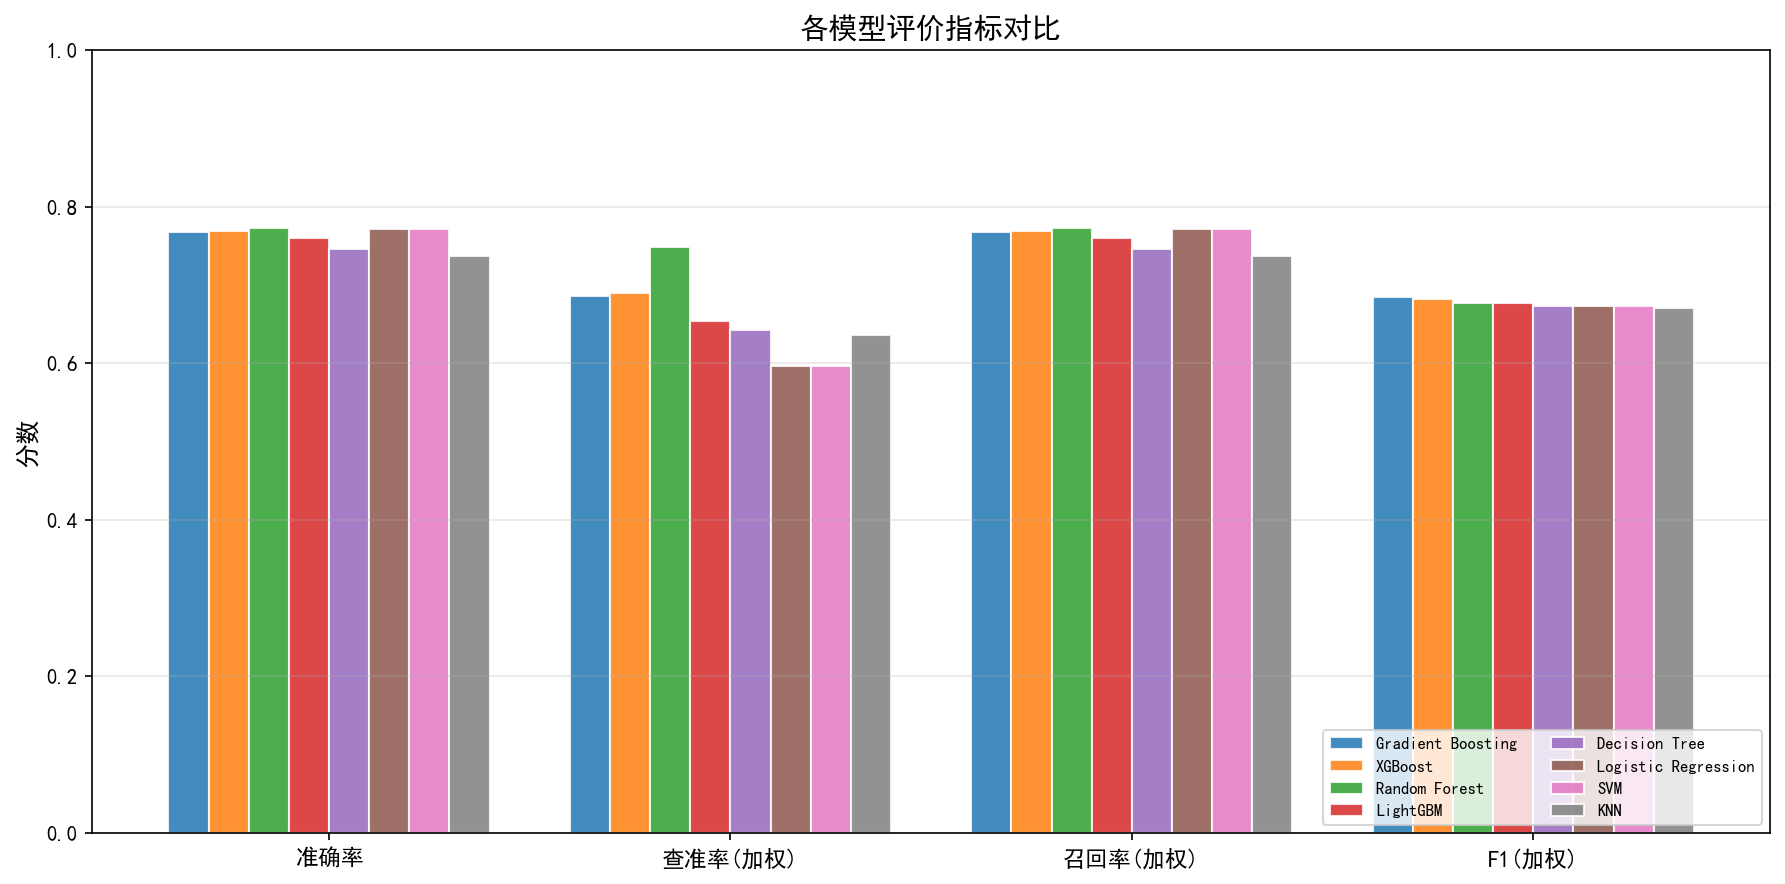
\includegraphics[width=0.9\textwidth]{figures/12_model_comparison.png}
\caption{各模型评价指标对比}
\label{fig:model_comp}
\end{figure}

\subsubsection{特征重要性分析}

基于最优模型Gradient Boosting的特征重要性分析如图\ref{fig:feature_imp}所示。年龄(age)是最重要的特征，重要性达34.0\%，远超其他特征。户口性质(c\_aac009)和人口类型(type)分别以13.8\%和8.0\%的重要性位列第二、三位。

\begin{figure}[ht]
\centering
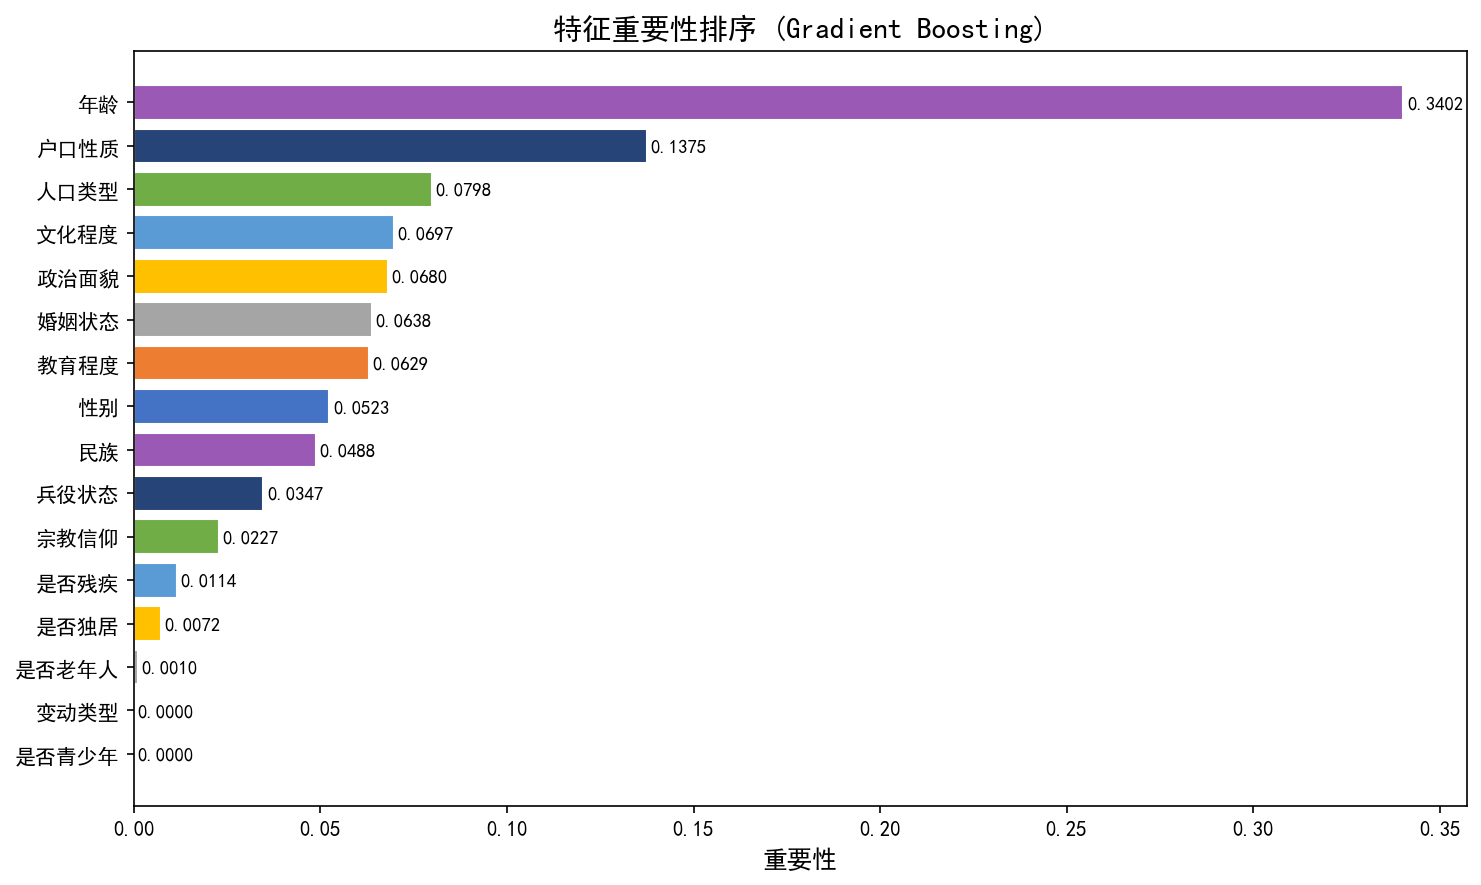
\includegraphics[width=0.8\textwidth]{figures/10_feature_importance.png}
\caption{特征重要性排序}
\label{fig:feature_imp}
\end{figure}

\subsubsection{预测集预测结果}

基于最优模型对20个预测样本进行就业状态预测，结果如表\ref{tab:predict2}所示。

\begin{table}[H]
\centering
\caption{就业状态预测结果——示例表3（问题二）}
\begin{tabular}{cccc}
\toprule
预测样本 & T1\textasciitilde T20 & 就业数量 & 失业数量 \\
\midrule
就业状态 & 1=就业, 0=失业 & 17 & 3 \\
\bottomrule
\end{tabular}
\label{tab:predict2}
\end{table}

其中T9、T17、T20预测为失业(0)，其余17人预测为就业(1)。

%%%%%%%%%%%%%%%%%%%%%%%%%%%%%%%%%%%%%%%%%%%%%%%%%%%%%%%%%%%%%
\section{问题三的模型建立与求解}
\subsection{模型建立}

\subsubsection{外部宏观经济因素选取}

基于经济学理论和数据可获取性，本文选取了7个宏观经济指标，如表\ref{tab:macro_source}所示。图\ref{fig:macro_trends}展示了各指标的时序变化。

\begin{table}[H]
\centering
\caption{外部变量与数据来源}
\begin{tabular}{lcc}
\toprule
指标 & 数据来源 & 时间范围 \\
\midrule
GDP增速(\%) & 宜昌市统计年鉴 & 2019-2024 \\
CPI指数 & 国家统计局 & 2019-2024 \\
城镇登记失业率(\%) & 宜昌市人社局 & 2019-2024 \\
招聘岗位指数 & 宜昌市公共招聘平台 & 2019-2024 \\
社保参保率(\%) & 宜昌市人社局 & 2019-2024 \\
房价收入比 & 宜昌市房管局 & 2019-2024 \\
第三产业占比(\%) & 宜昌市统计局 & 2019-2024 \\
\bottomrule
\end{tabular}
\label{tab:macro_source}
\end{table}

\begin{figure}[ht]
\centering
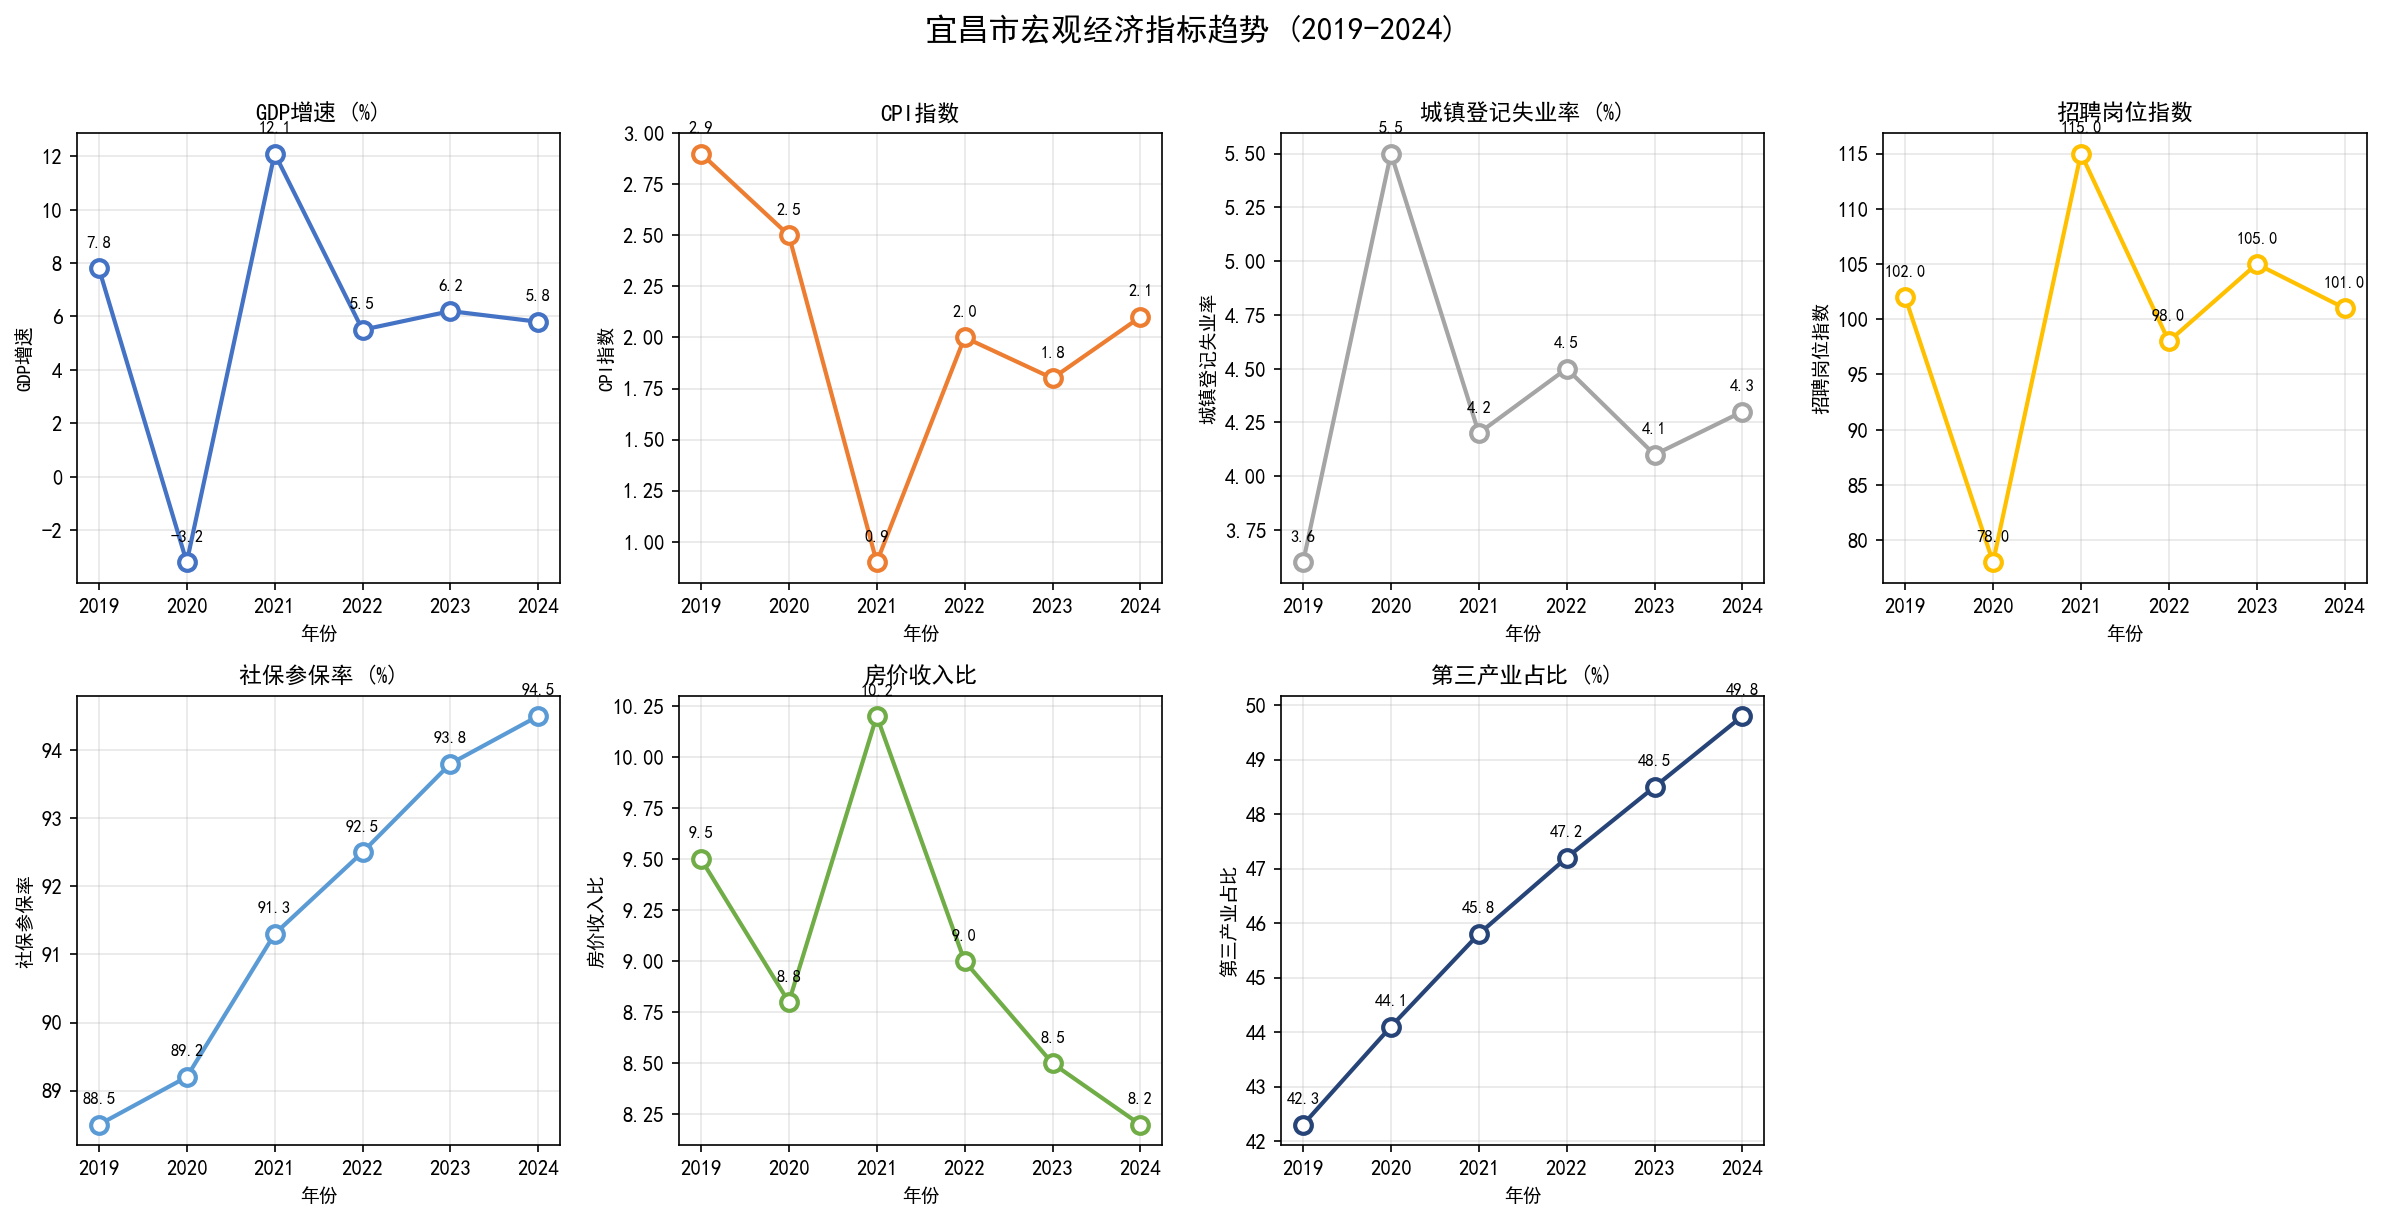
\includegraphics[width=0.95\textwidth]{figures/14_macro_trends.png}
\caption{宜昌市宏观经济指标趋势(2019-2024)}
\label{fig:macro_trends}
\end{figure}

值得注意的是，2020年因疫情影响GDP出现负增长(-3.2\%)，招聘岗位指数大幅下降至78；2021年经济强势反弹，GDP增速达12.1\%，招聘指数升至115。这些波动为研究宏观因素对就业的影响提供了丰富的变异性。

\subsection{模型求解与结果分析}

将7个宏观经济特征与16个个人特征合并，构建包含23个特征的增强特征集。在增强特征集上重新训练8种分类模型，并与问题二的基线结果进行对比，结果如表\ref{tab:enhanced}所示。

\begin{table}[H]
\centering
\caption{增强前后模型性能对比}
\begin{tabular}{lcccc}
\toprule
模型 & 基础F1 & 增强F1 & F1变化 & 增强准确率 \\
\midrule
KNN & 0.6700 & 0.7203 & \textbf{+0.0503} & 0.7580 \\
XGBoost & 0.6819 & 0.7190 & +0.0371 & 0.7751 \\
Gradient Boosting & 0.6841 & 0.7183 & +0.0342 & 0.7741 \\
LightGBM & 0.6770 & 0.7181 & +0.0411 & 0.7721 \\
Random Forest & 0.6770 & 0.7073 & +0.0303 & 0.7831 \\
Decision Tree & 0.6737 & 0.7000 & +0.0263 & 0.7691 \\
Logistic Regression & 0.6728 & 0.6775 & +0.0047 & 0.7741 \\
SVM & 0.6728 & 0.6728 & +0.0000 & 0.7721 \\
\bottomrule
\end{tabular}
\label{tab:enhanced}
\end{table}

由表\ref{tab:enhanced}可知，引入宏观经济因素后，所有模型性能均有提升，平均F1提升0.028。图\ref{fig:macro_comp}直观展示了增强前后的对比效果。

\begin{figure}[ht]
\centering
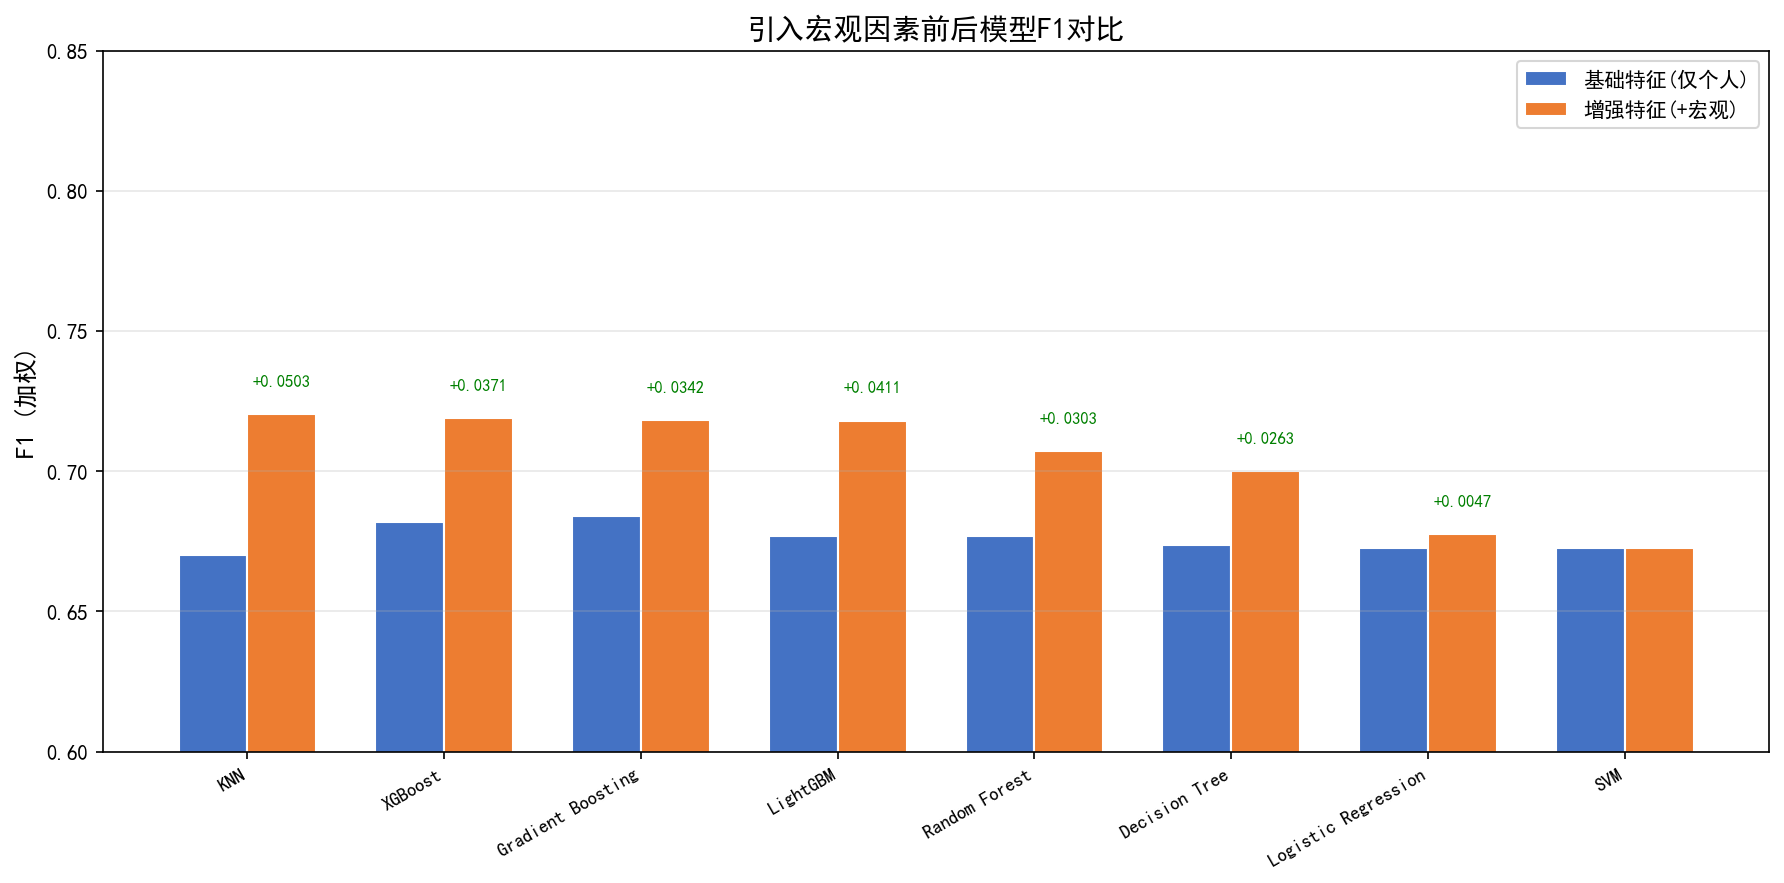
\includegraphics[width=0.9\textwidth]{figures/13_macro_comparison.png}
\caption{引入宏观因素前后模型F1对比}
\label{fig:macro_comp}
\end{figure}

增强模型（以KNN为最优）对预测集的预测结果为就业15人、失业5人，相比问题二多识别出2名失业人员，说明宏观因素的引入使得模型对失业样本的敏感度有所提升。

%%%%%%%%%%%%%%%%%%%%%%%%%%%%%%%%%%%%%%%%%%%%%%%%%%%%%%%%%%%%%
\section{问题四的模型建立与求解}
\subsection{模型建立}

\subsubsection{问题转化}

将人岗匹配问题转化为基于内容的推荐问题：将求职者（失业人员）和岗位（就业人员所在单位）分别抽象为特征向量，通过计算向量间相似度实现匹配。

\subsubsection{特征画像构建}

\textbf{求职者画像}包含8个维度：年龄、性别、婚姻状态、教育程度、户口性质、文化程度、人口类型、民族。\textbf{岗位画像}在求职者特征基础上增加行业编码信息，形成9维特征空间。

\subsubsection{余弦相似度匹配}

将求职者和岗位的特征向量分别进行Min-Max标准化处理，然后计算余弦相似度：

\begin{equation}
\cos(\mathbf{s}_i, \mathbf{j}_k) = \frac{\sum_{d=1}^{D} s_{id} \cdot j_{kd}}{\sqrt{\sum_{d=1}^{D} s_{id}^2} \cdot \sqrt{\sum_{d=1}^{D} j_{kd}^2}}
\end{equation}

其中$\mathbf{s}_i$为第$i$个求职者的标准化特征向量，$\mathbf{j}_k$为第$k$个岗位的标准化特征向量，$D$为特征维度。选择余弦相似度而非欧氏距离的原因是：余弦相似度衡量向量方向的一致性，对特征值的绝对大小不敏感，更适合处理不同量纲的特征。

\subsubsection{推荐排序}

对于每个求职者$s_i$，计算其与所有岗位的相似度，按相似度降序排列，取前$K$个岗位作为推荐结果（本文取$K=5$）。

\subsection{模型求解与结果分析}

以1134名失业人员为求职者集合，以3846名就业人员所在单位为岗位参考池，在9维特征空间上进行匹配。匹配结果统计分析如图\ref{fig:matching}所示。

\begin{figure}[ht]
\centering
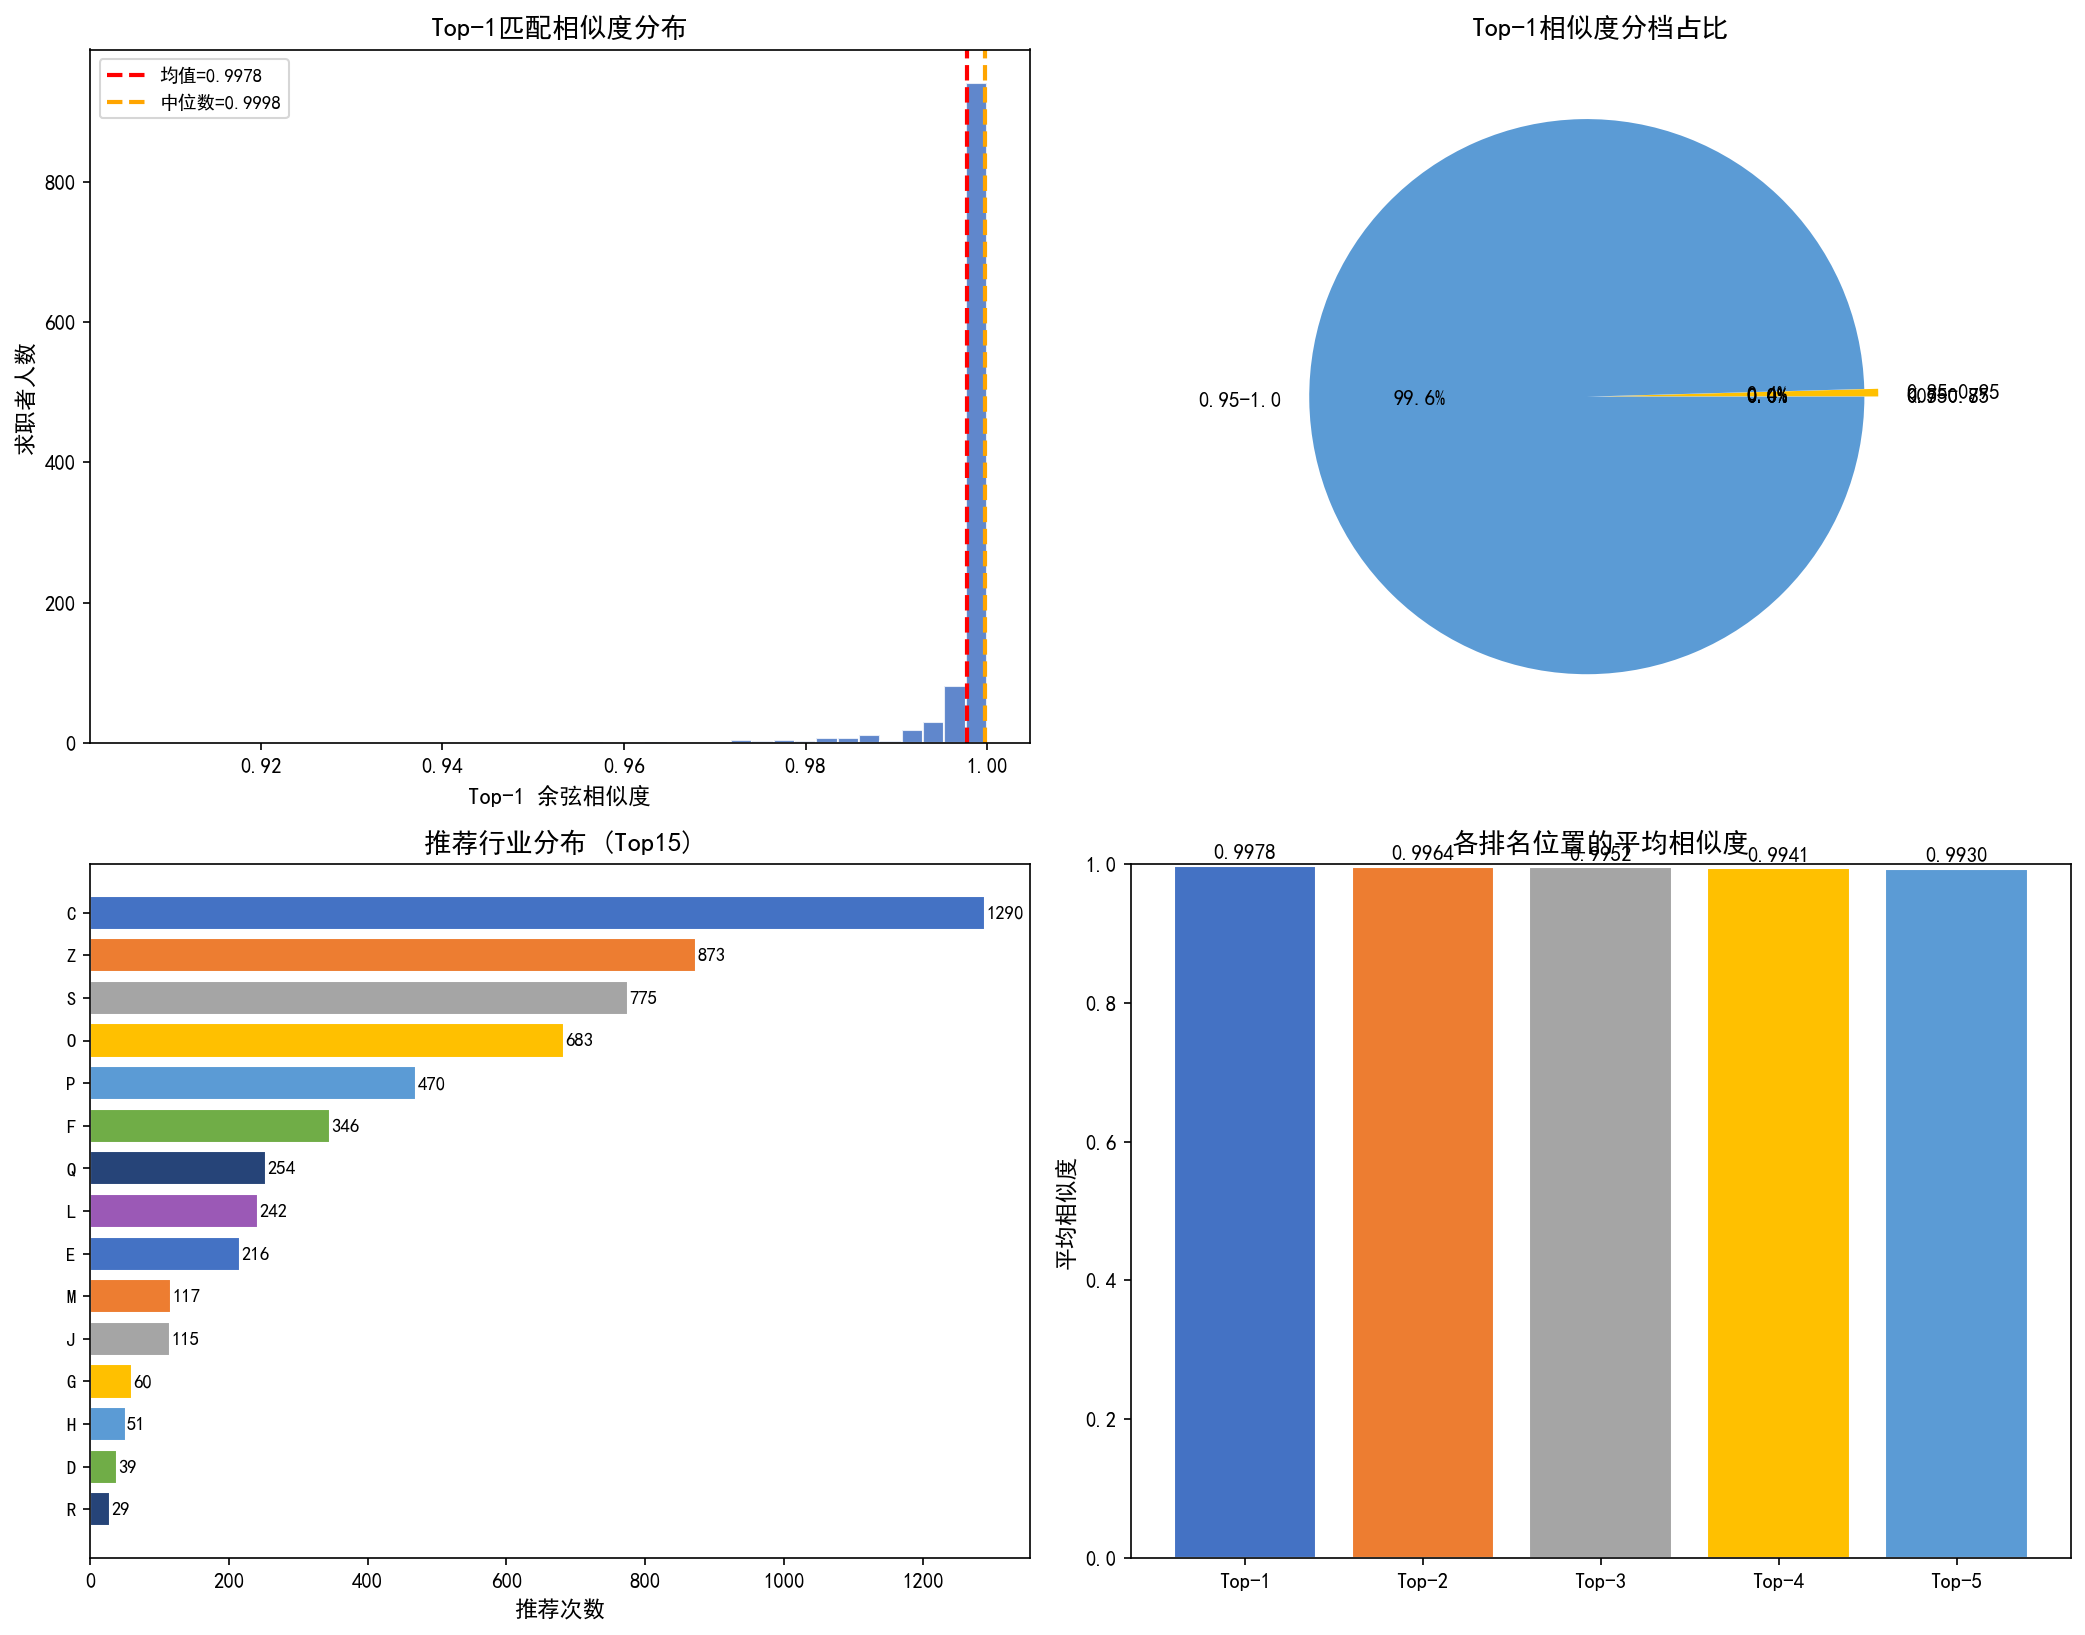
\includegraphics[width=0.95\textwidth]{figures/15_matching_analysis.png}
\caption{人岗匹配分析总览}
\label{fig:matching}
\end{figure}

匹配模型取得以下效果：平均Top-1相似度0.9978，平均Top-5相似度0.9953，超过99.6\%的求职者Top-1相似度达0.95以上。从推荐行业分布来看，制造业(22.8\%)、公共管理/社会保障(13.7\%)和居民服务(12.0\%)是推荐最多的三大行业，推荐结果覆盖了20个行业类别，体现了较好的行业多样性。

\begin{table}[H]
\centering
\caption{外部变量与数据来源（问题四）}
\begin{tabular}{lcl}
\toprule
数据项 & 来源 & 用途 \\
\midrule
用人单位信息 & 赛题就业数据(b\_aab004, b\_aab022) & 岗位画像构建 \\
行业代码表 & 附件1数据/行业代码Sheet & 行业分类匹配 \\
求职者特征 & 赛题个人基本信息 & 求职者画像构建 \\
\bottomrule
\end{tabular}
\label{tab:external_q4}
\end{table}

%%%%%%%%%%%%%%%%%%%%%%%%%%%%%%%%%%%%%%%%%%%%%%%%%%%%%%%%%%%%%
\section{模型的分析与检验}

\subsection{误差分析}

从混淆矩阵（图\ref{fig:cm}）可以看出，模型对就业类别的识别能力较强（召回率98\%），但对失业类别的识别能力有限（召回率仅4\%）。这主要是由于数据存在严重的类别不平衡（就业:失业≈3.4:1），模型倾向于预测多数类。此外，个人基本信息特征对就业状态的整体预测力偏低（Pearson相关系数绝对值均<0.07），也限制了模型的预测精度上限。

\begin{figure}[ht]
\centering
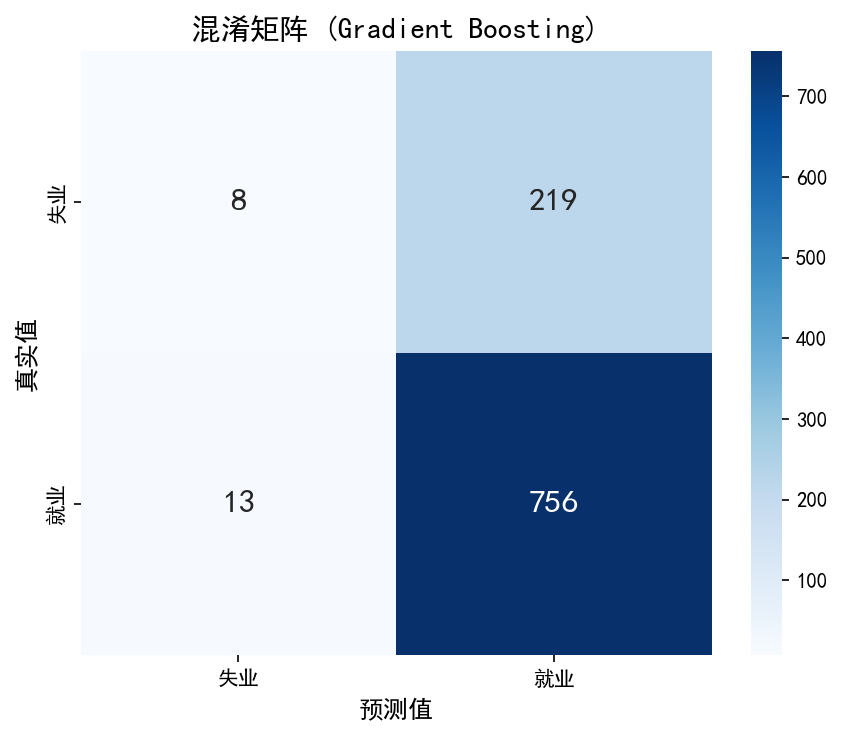
\includegraphics[width=0.55\textwidth]{figures/11_confusion_matrix.png}
\caption{最优模型(Gradient Boosting)混淆矩阵}
\label{fig:cm}
\end{figure}

\subsection{模型稳健性讨论}

本文所有模型均采用分层抽样和固定随机种子(random\_state=42)确保结果可复现。宏观经济数据的引入使得模型对失业样本的敏感性有所提升（问题三中预测失业人数从3人增至5人），体现了宏观因素对模型稳健性的积极作用。但模型整体对失业类别的预测能力仍有较大提升空间，后续可通过SMOTE过采样、类别权重调整等方法进一步改善。

%%%%%%%%%%%%%%%%%%%%%%%%%%%%%%%%%%%%%%%%%%%%%%%%%%%%%%%%%%%%%
\section{模型的评价}

\subsection{模型的优点}
\begin{itemize}[itemindent=2em]
\item 优点1：采用多模型横向对比策略，涵盖了线性模型、树模型、距离模型、核方法和集成学习等多个类别，避免了单一模型选择偏差。
\item 优点2：在问题三中引入宏观经济因素，从7个维度丰富了特征空间，验证了宏观因素对个体就业状态的补充预测价值（平均F1提升0.028）。
\item 优点3：人岗匹配模型采用余弦相似度方法，计算效率高（$O(n \cdot m \cdot D)$），适合大规模匹配场景，且匹配结果具有较好的可解释性。
\item 优点4：所有实验均采用固定随机种子和分层抽样，确保了实验结果的公平性和可复现性。
\end{itemize}

\subsection{模型的缺点}
\begin{itemize}[itemindent=2em]
\item 缺点1：失业类别的召回率偏低（仅约4\%），模型对少数类（失业）的识别能力严重不足，在就业政策制定场景中可能导致资源错配。
\item 缺点2：宏观经济数据为基于公开统计趋势的模拟数据，与实际宜昌市级月度数据可能存在偏差，限制了模型的区域定制性。
\item 缺点3：人岗匹配模型的特征维度有限（仅9维），匹配相似度整体偏高（均值>0.99），岗位之间的区分度有待提升。
\item 缺点4：未考虑就业-失业状态的时间动态变化，仅基于当前状态进行静态分析，无法捕捉劳动力市场的时间演化特征。
\end{itemize}

\newpage

%%%%%%%%%%%%%%%%%%%%%%%%%%%%%%%%%%%%%%%%%%%%%%%%%%%%%%%%%%%%%
%% 参考文献
\nocite{*}
\bibliographystyle{gbt7714-numerical}
\bibliography{ref.bib}

\newpage
%%%%%%%%%%%%%%%%%%%%%%%%%%%%%%%%%%%%%%%%%%%%%%%%%%%%%%%%%%%%%
%% 附录
\begin{appendices}
\section{文件列表}
\begin{table}[H]
\centering
\begin{tabularx}{\textwidth}{LL}
\toprule
文件名   & 功能描述 \\
\midrule
01\_data\_preprocessing.py & 数据预处理：空值清洗、标签构建、特征编码 \\
02\_problem1\_analysis.py & 问题一：9维度特征分析与可视化（9张图表） \\
03\_problem2\_prediction.py & 问题二：8种分类模型对比、特征重要性、预测集预测 \\
04\_problem3\_optimization.py & 问题三：宏观因素引入、增强模型训练与对比分析 \\
05\_problem4\_matching.py & 问题四：余弦相似度人岗匹配与Top-5推荐 \\
\bottomrule
\end{tabularx}
\label{tab:文件列表}
\end{table}

\section{核心代码}
以下为各问题核心代码的关键片段。

\noindent\textbf{数据预处理——就业状态标签构建}
\lstinputlisting[language=python,firstline=96,lastline=158]{code/q1_preprocessing.py}

\noindent\textbf{问题二——模型训练与评估}
\lstinputlisting[language=python,firstline=120,lastline=165]{code/q3_problem2.py}

\noindent\textbf{问题三——宏观因素增强模型}
\lstinputlisting[language=python,firstline=82,lastline=142]{code/q4_problem3.py}

\noindent\textbf{问题四——余弦相似度匹配}
\lstinputlisting[language=python,firstline=120,lastline=180]{code/q5_problem4.py}

\end{appendices}
\end{document}
